% options:
% thesis=B bachelor's thesis
% thesis=M master's thesis
% czech thesis in Czech language
% english thesis in English language

\documentclass[thesis=M,czech]{FITthesis}[2012/04/01]

\usepackage[utf8]{inputenc} % LaTeX source encoded as UTF-8

\usepackage{graphicx} %graphics files inclusion
% \usepackage{amsmath} %advanced maths
% \usepackage{amssymb} %additional math symbols

\usepackage{dirtree} %directory tree visualisation
\usepackage{multicol} %multi column support
%\usepackage{nameref} %referencing whole name

% tento kod zpusobi, ze cokoli uzavrene ve znacich || se vysazi jako kod
\usepackage{fancyvrb}
\usepackage{listings} %zdrojove kody
\usepackage{amsmath}

\usepackage{float}
%\usepackage{color} %colorbox

\lstdefinestyle{custom}{
  belowcaptionskip=1\baselineskip,
  breaklines=true,
  frame=L,
  xleftmargin=\parindent,
  showstringspaces=false,
  %columns=fixed,
  basicstyle=\footnotesize\ttfamily,
  % keywordstyle=\bfseries\color{green!40!black},
  % commentstyle=\itshape\color{purple!40!black},
  % identifierstyle=\color{blue},
  % stringstyle=\color{orange},
}

\DefineShortVerb{\|}

% % list of acronyms
% \usepackage[acronym,nonumberlist,toc,numberedsection=autolabel]{glossaries}
% \iflanguage{czech}{\renewcommand*{\acronymname}{Seznam pou{\v z}it{\' y}ch zkratek}}{}
% \makeglossaries% Z uživatelského hlediska je velmi výhodné před nákupem zboží prozkoumat trh pomocí internetových srovnávačů. Zatím ovšem není snadno dostupná služba, která by uživateli umožnila vytvořit si hypotetický seznam zboží, které zvažuje koupit.

% *Vytvořte rešerši stávajících systémů zabývajících se organizací nákupních seznamů.
% *Zjistěte možnosti a strategii napojení na systémy zabývající se srovnáním a sledováním cen.
% *V souladu s touto rešerší poté analyzujte, navrhněte a implementujte webovou aplikaci, která bude umožňovat přidávat, sledovat, prioritizovat a kategorizovat zboží, zobrazovat jeho cenu a její vývoj.
% *Webovou aplikaci implementujte v jazyce Ruby ve vhodném frameworku.
% *Pro prioritizaci navrhněte a implementujte vhodné algoritmy.
% *API webové aplikace bude navrženo s ohledem na budoucí integraci s dalšími systémy (např. srovnávače cen apod.).

\newcommand{\tg}{\mathop{\mathrm{tg}}} %cesky tangens
\newcommand{\cotg}{\mathop{\mathrm{cotg}}} %cesky cotangens

% % % % % % % % % % % % % % % % % % % % % % % % % % % % % % 
% ODTUD DAL VSE ZMENTE
% % % % % % % % % % % % % % % % % % % % % % % % % % % % % % 

\department{Katedra softwarového inženýrství}
\title{Webová aplikace pro správu a organizaci \newline nákupního seznamu}
\author{Tomáš Vik} %jméno autora bez akademických titulů
\authorWithDegrees{Bc. Tomáš Vik} %jméno autora včetně akademických titulů
\supervisor{Ing. Jiří Hunka}
\acknowledgements{Děkuji svému vedoucím práce Jiřímu Hunkovi za čas strávený konzultacemi a korekturou této práce. Děkuji svým rodičům, že mě vychovali a podporovali mě. A poté děkuji všem svým přátelům, kteří mi zpřijemňovali má vysokoškolská léta. Jmenovitě díky Bukáši, Vejvisi, Tomaassi, Medvěde, Pinokio, Váco, Sethe, Máro, Eliško, Sobe, Zůzo, Nováku, Stanely, Gulo, Kájo, Terko a Káťo.}
\abstractCS{Práce pojednává o problematice nákupních seznamů. Nejdříve prozkoumává současný trh těchto seznamů a systémů srovnávání cen zboží. Následně je navržena a implementována webová aplikace, která staví na tomto průzkumu. Při návrhu i implementaci je kladen důraz na jednoduchost uživatelského rozhraní. V závěru práce jsou provedeny uživatelské testy aplikace.}
\abstractEN{This thesis is concerned with shopping lists. In the first part of the thesis several already copmleted applications are described. Then web application is designed and implemented on the informations mentioned above. Application design is focused on user interface. Afterwards the application is tested by users.}
\placeForDeclarationOfAuthenticity{V~Praze}
\keywordsCS{seznam, srovnávání zboží, prioritizace, uživatelské rozhraní}
\keywordsEN{list, goods comparsion, prioritization, user interface}

%namedlabel control sequence for easy referencing of list items
\makeatletter
\def\namedlabel#1#2{\begingroup
    #2%
    \def\@currentlabel{#2}%
    \phantomsection\label{#1}\endgroup
}
\makeatother

\begin{document}

% \newacronym{CVUT}{{\v C}VUT}{{\v C}esk{\' e} vysok{\' e} u{\v c}en{\' i} technick{\' e} v Praze}
% \newacronym{FIT}{FIT}{Fakulta informa{\v c}n{\' i}ch technologi{\' i}}

% !TEX root = ../DP_Vik_Tomas_2013.tex
\begin{introduction}
V dnešní době je běžné, že se zákazník před koupí produktu informuje na internetu na cenu v různých obchodech. Dříve musel na internetu použít běžný fulltextový vyhledávač a každý nalezený výsledek produktu musel rozkliknout a nalézt cenu umístěnou na stránce obchodu.

Protože se jedná o relativně složitý proces, vznikly tzv. systémy pro srovnávání cen. Ty odstraňují nutnost hledat cenu výrobku v různých zdrojích. Díky tomu může zákazník přijít na stránku srovnávače cen, nalézt produkt, který chce koupit a poté na jedné přehledné stránce vidí nejen informace o produktu, ale také srovnání cen ve všech srovnávači dostupných obchodech.

Přesto že srovnávání cen je pro zákazníka usnadnění. Cílem této práce je poskytnou další kroky pro zjednodušení nákupu. Práce si klade za cíl navrhnout a vytvořit aplikaci, do které bude zákazníkovi umožněno vložit seznam zboží, které si přeje zakoupit. Takový seznam už některé srovnávače také podporují, ne však s dostatečnou funkcionalitou.

Uživatel bude mít možnost toto zboží (ve zbytku práce nazývané přání) v seznamu kategorizovat, prioritizovat a různými způsoby upravovat. Aplikace dále nejen že bude u těchto přání zobrazovat vývoj ceny, ale navíc dokáže uživatele upozornit na výraznou změnu v tomto vývoji.

V práci budou nejprve detailně zpracovány vlastnosti aplikací s podobnou myšlenkou a dále vlastnosti srovnávačů cen. Na zákaldě této rešerše bude navržena samotná aplikace. Při návrhu bude kladen důraz především na návrh grafického uživatelského rozhranní, které by mělo být intuitivní a usnadňovat uživateli co nejvíce jeho práci.

Dále je krátce popsána zajímavá část implementace a na koneci práce je uživatelské vyhodnocení návrhu grafického rozhraní.
\end{introduction}
% !TEX root = ../DP_Vik_Tomas_2013.tex
% pokyny
% Z uživatelského hlediska je velmi výhodné před nákupem zboží prozkoumat trh pomocí internetových srovnávačů. Zatím ovšem není snadno dostupná služba, která by uživateli umožnila vytvořit si hypotetický seznam zboží, které zvažuje koupit.

% *Vytvořte rešerši stávajících systémů zabývajících se organizací nákupních seznamů.
% *Zjistěte možnosti a strategii napojení na systémy zabývající se srovnáním a sledováním cen.
% *V souladu s touto rešerší poté analyzujte, navrhněte a implementujte webovou aplikaci, která bude umožňovat přidávat, sledovat, prioritizovat a kategorizovat zboží, zobrazovat jeho cenu a její vývoj.
% *Webovou aplikaci implementujte v jazyce Ruby ve vhodném frameworku.
% *Pro prioritizaci navrhněte a implementujte vhodné algoritmy.
% *API webové aplikace bude navrženo s ohledem na budoucí integraci s dalšími systémy (např. srovnávače cen apod.).
%
% - optimalizace na mobilni prohlizece, autocomplete nefunguje, drag'n drop
% - pridat detail do pridani prani
% - nemuzes hledat vec kterou nevis
% - registrace uzivatele
% - neprihlaseny zacina vyhledavanim
% - pri zavreni okna upozornit ze jsou neulozena prani
% - co se deje, pokud tam bude vice prani? - pokud se pridava prani, co se stane kdyz dojde prostor
% - jak dokazu reagovat na chybu datovyho zdroje - mit vyreseno
% - nabizet uzivatelum hlaseni chyb
% - kompatibilita s prohlizecema
% - co uzivateli nabidnu kdyz se vec nenajde - prazdna obrazovka bez vysledku vyhledavani
% - proc ne/ano trendy prani

% - vyvoj@jagu.biz - Michal Přibyl - Oponent - zkontaktovat
% - pavel žikovský - nechat si zkonzultovat návrh uživatelského rozhranní - do zítra urgovat
% - task graph do přílohy
% - jasně odůvodnit na začátku návrhu/konci rešerše
% - počítat s tím že aplikace je jednoduchá a obhájit proč je jednoduchá
% - přímo citovat z kapitoly 20 prani - neni obor IT
% - úvést že nákupní seznam je v mém pojetí brán jako seznam přání
% - sledovani ceny
% - nemusí obsahovat finální screeny
\chapter{Rešerše}
První kapitola je věnovaná popisu problematiky této práce a přehledu aplikací, ktere řeší stejné nebo podobné problémy.
Nejdříve se zabývá přímými konkurenty výsledné aplikace. Zde je shrnuta funkcionalita webových aplikací, které umožňují organizaci nákupních seznamů.
Dále se zabývá aplikacemi, které mají nějakou významnou funkčnost vhodnou pro výslednou aplikaci. Jedná se o aplikace, které se nějakou svojí částí specializují na organizaci informací. Konec kapitoly je věnován technologickému aspektu práce. Budou shrnuty technologie, na kterých je v dnešní době možné postavit webové aplikace.
Na konci každé podkapitoly budou shrnuty slabé a silné stránky jednotlivých technologií.

\section{Nákupní seznamy}
V následujících sekcích je popsána funkčnost hotových aplikací zabývajících se organizací nákupního seznamu. Všechny zmíněné aplikace jsou již v produkci a jsou zaštítěny velkými internetovými společnostmi.

\subsection{Google ShoppingList}
Webová aplikace doplňující službu Google Nákupy. Podporuje jednoduché přidání zboží. U přidaných položek zobrazuje následující informace a umožňuje podle těchto informací i řadit položky na seznamu:
\begin{itemize}
\item \textbf{Datum přidání položky}
\item \textbf{Nejnižší aktuální cena} - Služba Google Nákupy má informace o ceně získané z většího množství obchodů. U věci na seznamu zobrazuje nejnižší možnou cenu. Jiná než tato cena nelze zobrazit.
\item \textbf{Hodnocení produktu}
\end{itemize}
Zboží přidané do seznamu se dělí do dvou kategorií resp. seznamů. První seznam se nazývá Shopping List a jedná se o privátní nákupní seznam. Položky v tomto seznamu se zobrazují puze uživateli, kterému seznam patří. Druhý seznam se nazývá seznam přání a je možné na něj zkopírovat odkaz. Tento odkaz následně uživatel odešle komukoli, s kým chce svůj seznam přání sdílet. Položky lze přesouvat mezi seznamy tlačítkem \emph{Sdílet}/\emph{Zrušit sdílení}.
Zboží v seznamu přání je primárně určeno pro ostatní uživatele, aby jej mohli koupit uživateli, který seznam přání vytvořil. Například jako vánoční, narozeninový, nebo svatební seznam přání. Seznam přání je vidět na obrázku \ref{fig:google-shoppinglist}

Další funkčnost, kterou nabízí tento seznam je:
\begin{itemize}
\item Přidání poznámky k položce - uživateli je umožněno přidat poznámku k položce na seznamu.  Tato poznámka je následně zobrazena u položky v hlavním přehledu.
\item Odebrání položky ze seznamu
\item Sdílení/Zrušení sdílení - viz. předchozí odstavec
\end{itemize}

\begin{figure}[htb]
\begin{center}
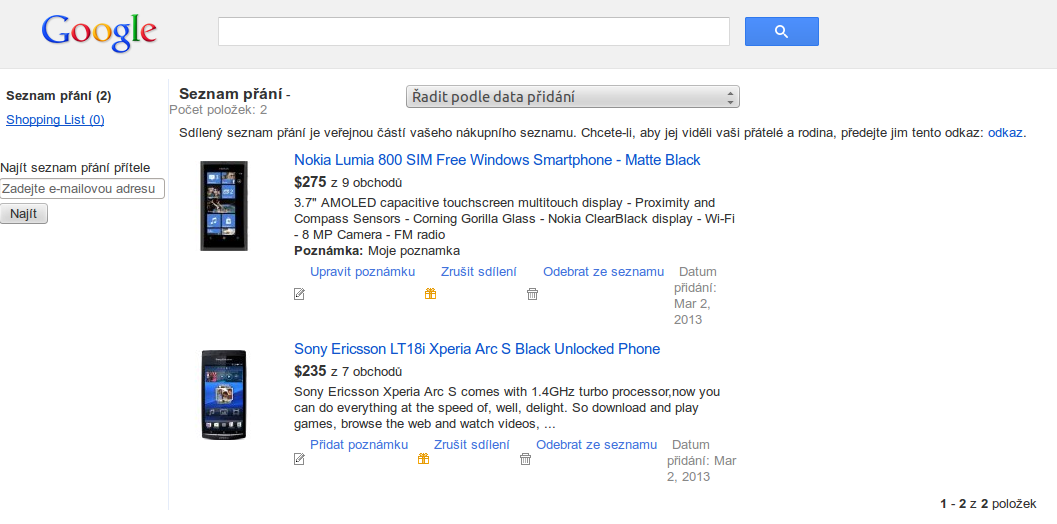
\includegraphics[width=120mm]{./pictures/google-shopping-list.png}
\caption{Google ShoppingList - základní obrazovka}
\label{fig:google-shoppinglist}
\end{center}
\end{figure}

\subsection{Amazon Wish List}
Amazon Wish List je funkcionalita poskytovaná komplementárně k internetovému obchodu Amazon.com. Služba umožňuje vytvářet a sdílet seznamy přání. Pro využívání této služby musí být uživatel přihlášen. Pokud se nepřihlášený uživatel pokusí přidat nějaký předmět do seznamu přání, je přesměrován na stránku přihlášení.

\subsubsection{Druhy přání}
Tato sekce se zabývá druhy přání ve službě Amazon Wish List. Přáním se v této službě rozumí tři věci:
\begin{itemize}
\item Produkt z internetového obchodu Amazon.com
\item Internetová stránka mimo Amazon.com
\item Nápad na přání (tzv. idea)
\end{itemize}

\paragraph{Produkt internetového obchodu Amazon.com}
\label{par:produkt-amazon}
Toto přání reprezentuje jedna k jedné produkt v internetovém obchodu Amazon.com. Toto přání vznikne tak, že přihlášený uživatel klikne na stránce produktu v obchodě Amazon.com na tlačítko \emph{Add To Wish List}. U takovéhoto přání se ukazuje minimální možná cena, popis i obrázek. Tedy maximální množství informací, které je aplikace schopna k přání uchovat.

\paragraph{Internetová stránka mimo Amazon.com}
Toto přání reprezentuje jakoukoliv internetovou stránku. Takovéto přáni vznikne jedině pomocí pluginu Amazon Wish List Button. O této funkcionalitě pojednává samostatná podkapitola \ref{sec:amazon-wishlist-button}.

\paragraph{Nápad na přání}
Nápad na přání je funkcionalita, která umožní uživateli zadat nápad na přání pouze jako text (název přání). Tento nápad se uloží mezi ostatní přání. Místo obrázku přání je ovšem zobrazen obrázek nalepovacího štítku a na něm je napsáno "I Want". Nápad na přání je vidět na obrázku \ref{fig:amazon-wishlist-idea}. Každý nápad na přání má u sebe tlačítko \emph{Top search results} které najde pro popis nápadu produkty z obchodu Amazon.com. Takto nalezené produkty je možné okamžitě přidávat do seznamu. Nápad na přání přitom v seznamu zůstává, dokud jej uživatel neodstraní.

\begin{figure}[htb]
\begin{center}

\includegraphics[width=100mm]{./pictures/amazon-wishlist-idea.png}
\caption{Nápad na přání v Amazon Wish List}
\label{fig:amazon-wishlist-idea}
\end{center}
\end{figure}

\subsubsection{Amazon Wish List Button}
\label{sec:amazon-wishlist-button}
Amazon Wish List poskytuje plugin\footnote{Také zásuvný modul - software, který nepracuje samostatně, ale jako doplňkový modul jiné aplikace a rozšiřuje její funkčnost.} do všech majoritních internetových prohlížečů\cite{website:amazon:plugin}. Po nainstalovani pluginu do prohlížeče si může uživatel přidat tlačítko \emph{Amazon Wish List Button} do ovládacího panelu prohlížeče. Po stisku tohoto tlačítka se otevře dialog. (Obrázek \ref{fig:amazon-wishlist-plugin})

\begin{figure}[htb]
\begin{center}
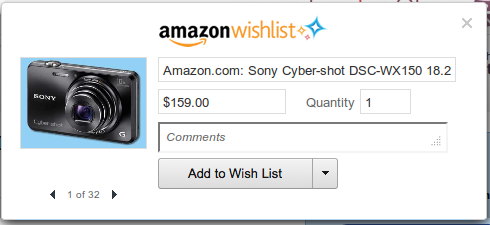
\includegraphics[width=100mm]{./pictures/amazon-wishlist-plugin.png}
\caption{Dialog zobrazeny po stisku Amazon Wish List Button}
\label{fig:amazon-wishlist-plugin}
\end{center}
\end{figure}

Přidat je možné buď produkt z obchodu Amazon.com. V tomto případě se načtou všechna data, která se u přání ukladájí, a není rozdíl v použití pluginu oproti stisknutí tlačítka "Add to Wish List" na stránce produktu (viz. kapitola \ref{par:produkt-amazon}).

Dále plugin podporuje funkci přidání přání v podobě jakékoli stránky. Tedy je možné přidat do Amazon Wish List například zboží z českého internetového obchodu. Jako obrázek k přání si uživatel může zvolit libovolý obrázek ze stránky. Jako název přání se použije titulek stránky\footnote{Obsah HTML tagu <title> ve zdrojovém kódu stránky}, popisek se k přání žádný nepřidává. Uživatel si ještě k přání muže doplnit cenu před tím než ho uloží do seznamu.

\subsection{WishList.com}
WishList.com je webová aplikace zaměřená primárně na vytváření seznamu přání. U každého seznamu podporuje sdílení a také podporuje nastavení události k seznamu a data této události. Většina seznamů má tyto hodnoty vyplněny a jsou to například seznamy přání k narozeninám, vánocům nebo seznam svatebních darů. Jako zdroj dat používá internetový srovnávač PriceGrabber.com, který je popsán v rešerši srovnávačů.

WishList.com neumožňuje přihlášení pomocí OpenID. Uživatel se může přihlásit pomocí svého Facebook účtu, nebo zaregistrovat klasickou metodou, kdy zadá svůj email, přihlašovací jméno a heslo.

Uživatel může vytvářet nové seznamy přání a nová přání. Při vytvoření nového seznamu zadává uživatel jeho název, obrázek, omezení přístupu (veřejný, pouze přátelé, soukromý), popis, osobní poznámky, osobu, která si věci přeje, název a datum události. Pouze název seznamu je povinné pole. Seznam je navíc možné zabezpečit heslem.

Při přidávání přání je možné zadat prodejce předmětu, název předmětu, popis předmětu, cenu, množství, prioritu, poznámky k přání, seznam přání do kterého bude přání přidáno, příjemce přání a poté URL produktu a URL obrázku produktu. Povinným polem je pouze název předmětu.

Vytvořený seznam je možné sdílet pomocí URL. Pokud si seznam prohlíží jiný uživatel než ten, který jej vytvořil, může si tento uživatel zarezervovat přání, což znamená že koupí předmět a dá jej uživateli, který si jej přál.

Seznam přání i jednotlivá přání je možné sdílet s ostatními uživateli pomocí tlačitka \emph{Share this WishList} resp \emph{Share this Wish}. Sdílení je možné pomocí služeb Facebook, Myspace, Google, Twitter, Email a dalších více než 300 sociálních služeb. Na sdílení je pravděpodobně použit nějaký plugin.

Aplikace WishList podporuje vyhledávání zboží pomocí více zmíněného PriceGrabber.com. Pokud má zboží pouze jednoho prodejce, přesměruje uživatele tlačítko \emph{Buy} u přání přímo na stránku prodejce. Jinak je uživatel přesměrován na stránku s výběrem prodejců. Tato stránka se nachází stále na WishList.

Po přidání přání, které bylo nalezeno vyhledáváním je uživateli zobrazena zpráva, která se ptá jestli chce uživatel opravdu čekat a nekoupí si své přání rovnou. Tato výzva je vidět na obrázku \ref{fig:wishlist-buynow}.

\begin{figure}[htb]
\begin{center}
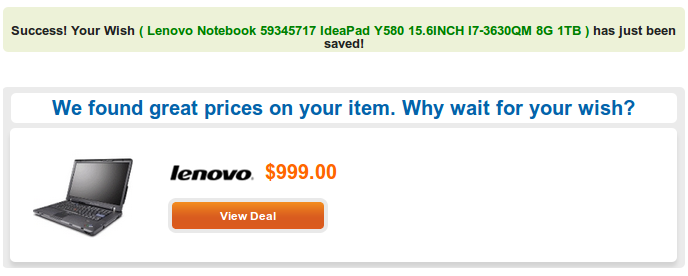
\includegraphics[width=100mm]{./pictures/wishlist-buynow.png}
\caption{Výzva k okamžitému zakoupení přání.}
\label{fig:wishlist-buynow}
\end{center}
\end{figure}

Přehled přání je vidět na obrázku \ref{fig:wishlist-wishlist}.

\begin{figure}[htb]
\begin{center}
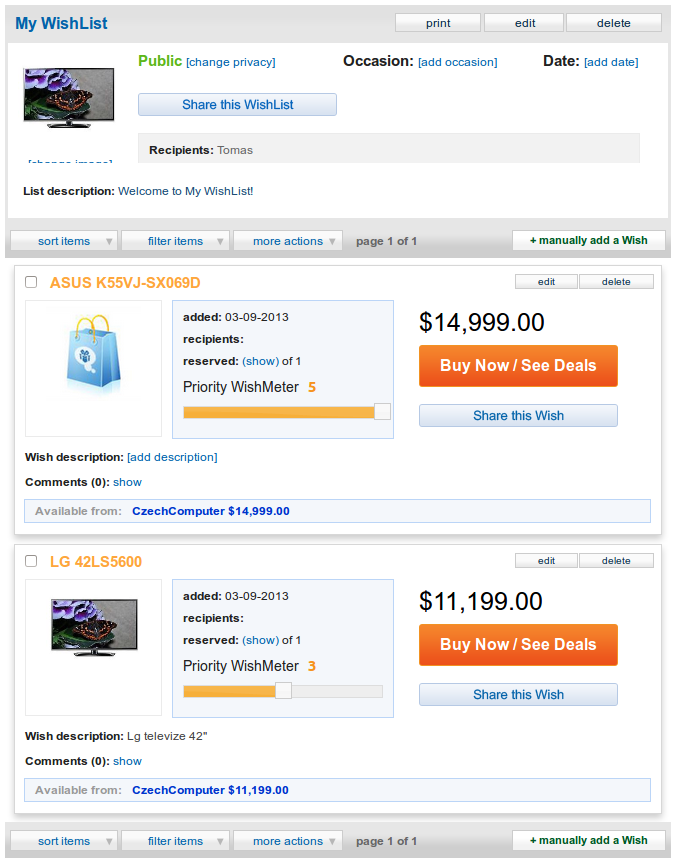
\includegraphics[width=100mm]{./pictures/wishlist-wishlist.png}
\caption{Hlavní přehled přání na stránce WishList.com}
\label{fig:wishlist-wishlist}
\end{center}
\end{figure}

\subsubsection{Nedostatky WishList.com}
Cena u přání jde zadat pouze v dolarech. WishList umožňuje vyhledat zboží pro přání u kterých není uvedena URL produktu, ale vyhledávání nefunguje kompletně, nenašlo nic pro výraz "iphone", pro který PriceGrabber (zdroj dat pro WishList) nalezne několik stovek výsledků.

\section{Srovnávače cen}
Tato kapitola poskytuje rešerši aplikací známých jako srovnávače cen, jejichž cílem je poskytnout uživateli širší pohled na trh. Tyto aplikace umožňují u jednoho produktu srovnat cenu v několika internetových obchodech. V rešerši jsou zpracovány jako potencionální zdroje dat pro výslednou webovou aplikaci.

\subsection{Standartní funkce všech srovnávačů}
V této sekci jsou popsány tři základní funkce, které podporují všechny zmíněné srovnávače cen. Lze říci že se jedná o funkce, které definují srovnávač cen jako takový.

\subsubsection{Vyhledávání}
Každý ze zmíněných vyhledávačů podporuje fultextové vyhledávání zboží\footnote{(z ang. full – celý, plný a text) speciální způsob vyhledávání informací v databázích nebo v textových souborech, které jsou obvykle předem připraveny, tj. indexovány, aby bylo možno nalézt libovolné slovo (řetězec znaků) v nejkratším možném čase.}. Toto vyhledávání probíhá nad databází veškerých výrobků, které aplikace (srovnávač) obsahuje. Vyhledávány jsou jednotlivé výrobky, u nichž jsou agregovány ceny z jednotlivých obchodů, tzn. že výrobek se zobrazí v ideálním případě\footnote{Produkt může mít v různých obdhodech různá jména, takové produkty se ne vždy podaří srovnávači agregovat.} pouze jednou, přesto že srovnávač má informace o několika obchodech, které jej poskytují.

Dále umožňují srovnávače vyhledávání po kategoriích. Na domovské stránce srovnávače je uživateli nabídnut seznam kategorií a významných podkategorií. Uživatel po rozkliknutí kategorie vidí vybrané zboží z dané kategorie a případně také podkategorie, pokud nějaké jsou.

Uživateli je také umožněno filtrovat zboží na základě jeho parametrů. Parametry podle kterých se filtruje se dají rozdělit na druhy:
\begin{itemize}
\item \textbf{Společné pro veškeré zboží.} Sem spadá například cena výrobku, nebo značka výrobce
\item \textbf{Rozlišné pro každou kategorii.} Zde se nacházejí parametry které dávají smysl pouze v dané kategorii. Např. velikost ohniska u objektivů nemá smysl nikde jinde. Stejně tak velikost uhlopříčky nemá smysl v kategoriích kde není žádné zobrazovací zařízení.
\end{itemize}

\paragraph{Databáze zboží}
Srovnávače cen plní svojí databázi zboží z dat od zákazníku. U porovnávaných srovnávačů je princip následující: Obchod, který chce, aby jeho zboží bylo vidět ve srovnávači, vystaví veřejně XML soubor, ve kterém je detailní popis každého produktu včetně informací jako způsob a doba doručení.\cite{website:heureka:registrace-obchodu}

\subsubsection{Srovnávání cen}
Každá aplikace podporuje srovnání cen u zobží. U většiny zboží v databázi je přiřazen větší počet obchodů. Díky shromáždění cen z jednotlivých obchodů je poté srovnávač schopný zobrazit u zboží nejnižší a nejvyšší cenu. U zboží je zároveň zobrazen přehled všech obhodů ve kterých je zboží nabízeno. Několik obchodů je zpravidla doporučeno srovnávačem. K tomu mohou mít obchody ještě seznam ocenění získaných srovnávačem.

Zpravidla je u obchodu zobrazena táké dostupnost zboží, případně cena dopravy. Díky těmto informacím uživatel okamžitě vidí kdy může zboží mít a kolik zaplatí navíc oproti ceně uvedené v obchodě.

Díky pravidelnému sledování cen zboží v obchodech má srovnávač chronologická data o ceně zboží. Díky této vlastnosti nabízí funcionalitu graf historie cen. V grafu je zanesena cena zboží řádově za několik uplynulých měsícu. Tento graf pomáhá uživateli v rozhodnutí o koupi. Uživatel vidí, zdali se cena právě nachází pod nebo nad dlouhodobým průměrem.

\subsubsection{Uživatelská zpětná vazba}
Srovnávače z pravidla umožňují uživatelům hodnotit obchody i zobží. U obchodů se hodnotí parametry jako dodací lhůta, přehledonost obchodu a kvalita komunikace. U zboží je výběr parametrů pro hodnocení jako při filtrování zboží podle atributů. V každé kategorii se hodnotí relevantní parametry zboží. 

Hodnocení většinou probíhá na principu jedné až pěti hvězdiček, případně shrnutí kladů a záporů.

Hodnocení produktu na srovnávači Heureka.cz je vidět na obrázku \ref{fig:heureka-hodnoceni-produktu}

\begin{figure}[htb]
\begin{center}
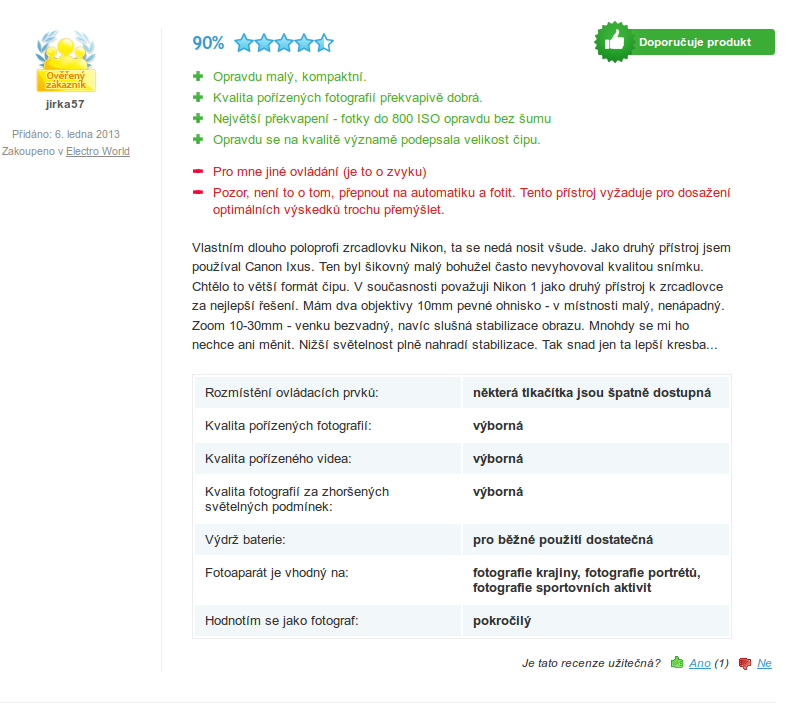
\includegraphics[width=100mm]{./pictures/heureka-hodnoceni-produktu.png}
\caption{Hodnocení produktu Nikon 1 J1 na srovávači Heureka.cz}
\label{fig:heureka-hodnoceni-produktu}
\end{center}
\end{figure}

\subsection{Heureka}
Interaktivní nákupní rádce Heureka.cz byl založen společností Miton v roce 2007, kdy ihned zaujmul zajímavým nápadem zkombinování mnoha užitečných možností do jednoho celku. Následně rozšiřuje svou působnost i na Slovensko a zakládá slovenskou verzi Heureka.sk (založena v r. 2008). \cite{website:wiki:heureka}

\subsubsection{Přidaná funkcionalita}
Další důležitou fukčností je hlídač ceny. Přihlášenému uživateli je umožněno na zboží nastavit hlídače ceny a poté co cena v nejlevnějším obchodě klesne pod zadanou částku, uživatel dostane email s upozorněním.

\begin{itemize}
\item \textbf{Záruka vrácení peněz u některých obchodů.} U smluvních partnerů 
\item Varování před obchody, které nedodržují své obchodní podmínky
\item Sledovaní slev a novinek na trhu
\end{itemize}
\subsection{Zboží.cz}
Zboží.cz je srovnávač cen vyvořený společností Seznam.cz. Na Zboží.cz je registrováno více než 16000 obchodů a více nže 62 milionu produktů. Denně navštíví srovnávač 180000 uživatelů a každý uživatel v průměru na stránce stráví 39 min.\cite{website:zbozi-about}
Zboží.cz je satelitní web společnosti Seznam.cz
\footnote{Satelitní web je rozšířená a propracovanější forma tzv. microsite (jinak také minisite či weblet), jde o speciální samostatný web plnící funkce, které se na hlavní webovou prezentaci nehodí, nebo s ní dokonce nesouvisejí.}
.
\subsubsection{Přidaná funkcionalita}
Zajímavou funckionalitou je srovnávání zboží. Uživatel má možnost přidat produkt do srovnání zboží pomocí tlažítka \emph{Přidat do porovnání} viz obrázek \ref{fig:zbozicz-srovnat}. Tím se zboží přidá do seznamu. Tento seznam obsahuje pro každý produkt jedne sloupec a v každém řádku je nějaká vlastnost produktu. Pokud produkt ve srovnání nemá danou vlastnost, je v dané buňce nápis \emph{Neznámý}.

\begin{figure}[htb]
\begin{center}

\includegraphics[width=40mm]{./pictures/zbozicz-srovnat.png}
\caption{Tlačítko pro srovnání zboží.}
\label{fig:zbozicz-srovnat}
\end{center}
\end{figure}

Výsledek takového srovnání je poté vidět na obrázku \ref{fig:zbozicz-srovnani}.

\begin{figure}[htb]
\begin{center}
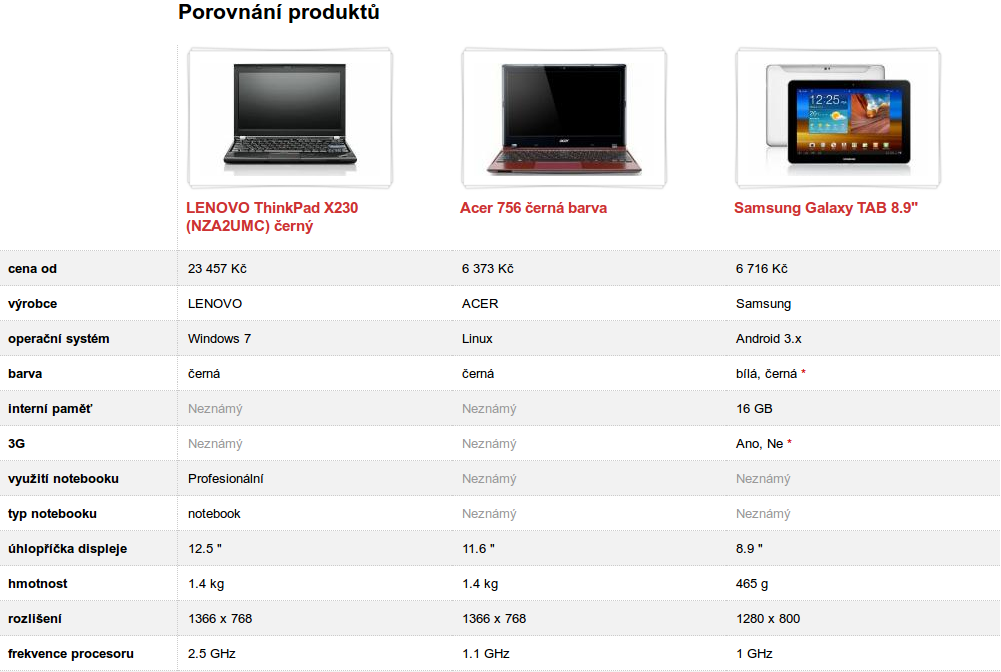
\includegraphics[width=130mm]{./pictures/zbozicz-srovnani.png}
\caption{Výsledek srovnání zboží na serveru Zboží.cz}
\label{fig:zbozicz-srovnani}
\end{center}
\end{figure}

\subsection{PriceGrabber}
PriceGrabber je služba pro srovnávání cen. Jejími partnery je více než 13000 prodejců. Poskytuje volně informace o milionech produktů ve více než 25 kategoriích. Společnost také slouží jako datový zdroj pro další prodejní služby jako AOL Shopping, Bing Shopping aj. \cite{website:wiki:pricegrabber}

Price grabber byl první srovnávač, který zahrnul informace o daních a poplatcích za přepravu do srovnávání. \cite{website:wiki:pricegrabber}

\subsubsection{Přidaná funkcionalita}
Price graber obsahuje funkčnost v čechách poprvé zavedenou portálem Slevomat.cz\footnote{Slevomat je český server hromadného nakupování založený Tomášem Čuprem, Petrem Bartošem a Romanou Sudovou.}. Tato funkčnost se nazýva "Local Deals" a umožňuje uživateli pořizovat zvýhodněné služby a/nebo zboží.

PriceGrabber obsahuje velké množství tzv. "Buying Guiedes" tedy příručky k nákupu, které poskytují základní rady a doporučení pro koupi daného typu zboží. Obsahuje tedy například příručku pro nákup klimatizace.

\section{Aplikace s žádanou funkčností}
Tato kapitola popisuje několik aplikací, které svým zaměřením nesplňují přímo podmínky této práce, ale část jejich funkcionality by byla pro výslednou aplikaci přínosem.

\subsection{Astrid}
\label{sec:astrid}
Astrid je aplikace pro správu úkolů. Mezi její klíčové funkce patří vytváření, úprava a kategorizace úkolů. Tato aplikace byla původně navržena pro mobilní zařízení a operační systém Android, nyní má aplikace také webové rozhranní, jehož funkcinalita je předmětem této kapitoly.

Základní obrazovku aplikace je možné vidět na obrázku \ref{fig:astrid}

\begin{figure}[htb]
\begin{center}
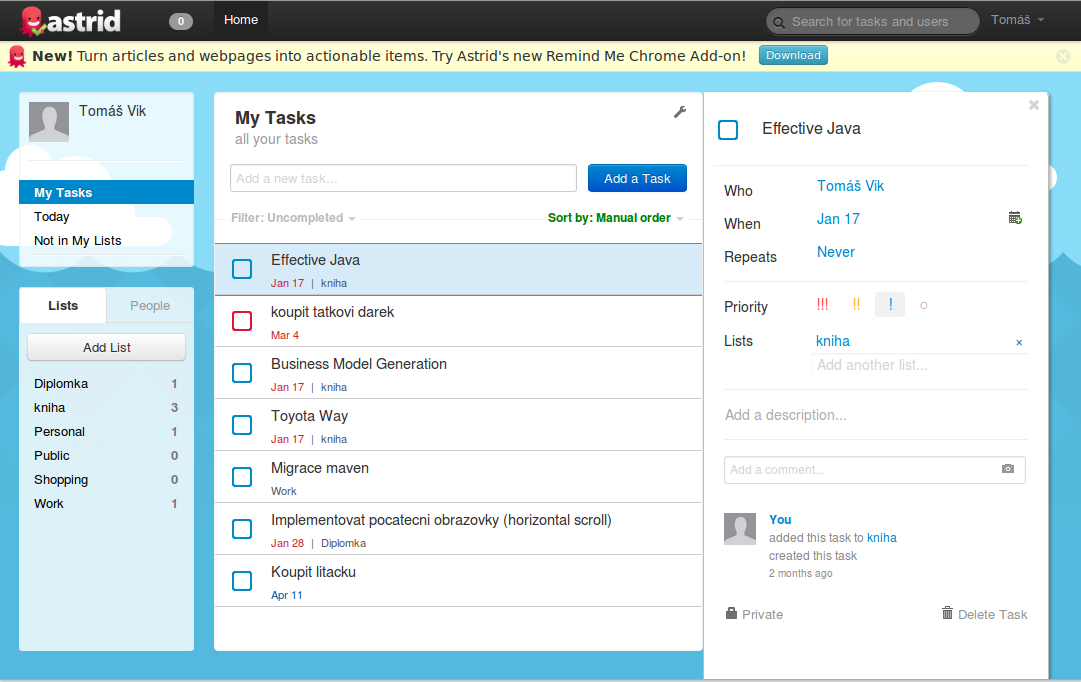
\includegraphics[width=130mm]{./pictures/astrid.png}
\caption{Základní strana webové aplikace Astrid.com}
\label{fig:astrid}
\end{center}
\end{figure}

Ná základní straně je vidět jednoduchost aplikace. Přidání úkolu proběhne pomocí vyplnění názvu úkolu a stisknutí tlačítka \emph{Add a Task}. Tím se úkol zobrazí v seznamu ostatních úkolů a jeho detaily už je pak možné nastavit stejně jako u všech ostatních úkolů.

Editace úkolu se provede kliknutím na daný úkol v seznamu. V pravé části obrazovky se zobrazí panel s detailními informacemi o úkolu.

Hlavní seznam úkolů je možné řadit pomocí několika kritérií. Mimo standardní kritéria jako priorita a datum přidání je možné řadit také manuálně (tzv. \emph{Manual order}). Uživatel může kliknout na položku na seznamu a přetáhnout ji mezi jakékoli 2 jiné položky, nebo na začátek/konec seznamu. Takto je uživateli umožněno seřadit si úkoly dle libosti.

Každý úkol náleží do 0-n seznamů. Tyto seznamy je možné libovolně výtvářet a mazat. Přidáváním přání do seznamů je uživateli umožněna další úroveň kategorizace. U každého seznamu se ukazuje panel s informacemi o aktuálních aktivitách v seznamu (např. vytvoření, dokončení a úprava úkolu).

Mazání přání probíhá pomocí tlačítka \emph{Delete Task} v panelu s informacemi o úkolu. Tímto tlačítkem se úkol okamžitě smaže, ale uživateli se zobrazí upozornění v horní části obrazovky. V tomto upozornění je také tlačítko na vrácení smazání přání viz. obrázek \ref{fig:astrid-undo}. Toto upozornění po několika málo vteřinách zmizí. Poté může uživatel obnovit přání ze seznamu akcí provedených nad seznamem přání.

\begin{figure}[htb]
\begin{center}

\includegraphics[width=130mm]{./pictures/astrid-undo.png}
\caption{Panel informující o smazání úkolu umožňuje vrátit operaci zpět}
\label{fig:astrid-undo}
\end{center}
\end{figure}


Pokud jsou mazané položky relativně nedůležité pro uživatele a manipuluje s nimi ve velkém (což je případ právě úkolů). Je toto vhodnější způsob než kalsický dialog pro potvrzení smazání. Uživatel v naprosté většině případů má v úmyslu úkol smazat, ale pokud to udělá omylem může smazání bezpečně vrátit. 

Aplikace umožňuje také poslat uživateli email s upozorněním na blížící se termín splnění přání.

Poslední zajímavá funkčnost je \emph{Remind Me button} tedy tlačítko, které si může jakýkoli uživatel umístit na webové stránky a pokud na něj klikne návštěvník této stránky, je mu automaticky přidán úkol do seznamu úkolů. HTML kód tlačítka se vytvoří pomocí jednoduchého formuláře, do kterého se zadá nadpis úkolu, za jak dlouho (popř. kdy) má být úklol splňěn, název internetové stránky, na které je tlačítko umístěno a URL které se úkolu týká.

Technicky je celá aplikace řešena pomocí AJAX. To znamená, že se stránka nenačítá znovu po každém kliknutí na tlačítko/odkaz, ale pouze se doplňují data do potřebných částí stránky. K určení cesty na stránce se používá tzv. identifikátor fragmentu\footnote{Krátký řetězec znaků označující zdroj, který je podřízený jinému, primárnímu, zdroji. Primární zdroj je určen URI, identifikátor fragmentu je od URI oddělen znakem \#.}. Frontend aplikace je postaven na technologii twitter bootstrap.
%https://twitter.com/astrid/status/222836247498985472

\section{Technologie pro vývoj aplikace}
Tato část rešerše se zabývá technologiemi, ve kterých je možné implementovat webovou aplikaci. V každé podkapitole je nejrpve popsán programovací jazyk a k němu následují nejpoužívanější frameworky pro implementaci webových aplikací.
\subsection{Java}
Java je objektově orientovaný programovací jazyk, který vyvinula firma Sun Microsystems a představila 23. května 1995.

Java je jedním z nejpoužívanějších programovacích jazyků na světě. Podle Tiobe indexu je Java nejpopulárnější programovací jazyk.[1] Díky své přenositelnosti je používán pro programy, které mají pracovat na různých systémech počínaje čipovými kartami (platforma JavaCard), přes mobilní telefony a různá zabudovaná zařízení (platforma Java ME), aplikace pro desktopové počítače (platforma Java SE) až po rozsáhlé distribuované systémy pracující na řadě spolupracujících počítačů rozprostřené po celém světě (platforma Java EE). Tyto technologie se jako celek nazývají platforma Java. Dne 8. května 2007 Sun uvolnil zdrojové kódy Javy (cca 2,5 miliónů řádků kódu) a Java bude dále vyvíjena jako open source.
\subsubsection{Spring MVC}
Spring MVC Web framework funguje na principu návrhového vzoru MVC. Tedy jasné oddělení perzistence, biznys logiky a prezentační vrstvy. Napříč těmito vrstvami je doménový model, tedy java třídy reprezentující datový model aplikace\cite{liu2006research}.

\begin{figure}[htb]
\begin{center}
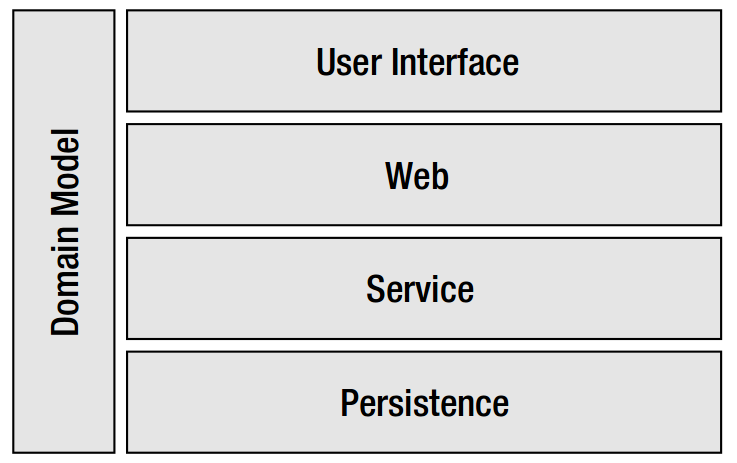
\includegraphics[width=50mm]{./pictures/spring-mvc-layers.png}
\caption{Aplikační vrstvy Spring MVC aplikace \cite{liu2006research}}
\label{fig:spring-mvc-layers}
\end{center}
\end{figure}

Jak název napovídá Spring MVC framework je postaven na aplikačním frameworku Spring. Využívá jeho základní mechanismy, jako Inversion Of Control kontejner a Dependency Injeciton.

Výhodou Spring MVC je, že je možné vybrat různé knihovny pro řešení specifických problémů aplikace. Např. knihovnu pro řešení prezistence (MyBatis, Hybernate), nebo knihovnu pro view (JSP, Velocity, FreeMarker, atd.)\cite{liu2006research}.

\subsection{Ruby}
Ruby je dynamický, reflexivní, objektově orientovaný programovací jazkyk, který kombinuje syntaxi inspirovanou jazykem Perl s funkcemi podobnými Smalltalku. Ruby je také ovlivněný jazyky Eiffel a Lisp. Ruby byl prvotně navržen a vyvinut v polovině devadesátých let minulého století japoncem Yukihiro "Matz" Matsumoto.

Ruby podporuje několik programovacích paradigmat. Mimo jiné funkcionální, objektově orientované, imperativní a reflektivní. Ruby má dynamické typování a automatickou správu paměti. Je tedy v mnohých aspektech podobný jazykům Smalltalk, Python, Perl, Lisp, Dylan, Pike a CLU.

Současná verze jazyka je 1.9.3.
\subsubsection{Ruby on Rails}
Ruby on Rails je framework pro vývoj webových aplikací napojených na databázi, používající návrhový vzor Model-view-controller. Vytvořil jej dánský programátor David Heinemeier Hansson při práci na projektu Basecamp.

Vše v Rails je založeno na jazyce Ruby. Na jazyce Ruby je založen Ajax v šablonách (view), odpovědi v controllerech i architektura aplikace v modelech obalujících databázi. Ke spuštění aplikace je třeba jen databáze.

Mezi základní princip Rails patří Konvence má přednost před konfigurací, tedy že programátor konfiguruje pouze ty části aplikace, které se liší od běžného nastavení. Vytvoří-li tedy např. model Person, aplikace bude data automaticky hledat v tabulce people. Chce-li, aby aplikace načítala data z tabulky staff, musí tak učinit výslovně.

Rails jsou postaveny na bázi návrhového vzoru Model-view-controller, který odděluje části aplikace zodpovědné za čtení a ukládání dat včetně manipulace s nimi (model), za zobrazení grafického rozhraní aplikace (view) a za část přijímající vstupy od uživatele a řídící zobrazení dat na výstupu (controller).

\subsubsection{Sinatra}
Sinatra je minimalistický framework\footnote{Zde se definice liší, například Alan Harris ve své publikaci Sinatra Up and Running píše, že sinatra není framework, ale podle mě definici tohoto slova naplňuje.} a doménově specifický jazyk\footnote{Doménově specifický jazyk je programovací jazyk, který je prostřednictvím vhodné abstrakce a výrazového slovníku zaměřen na omezenou, konkrétní problémovou doménu. V tomto případě jsou doménou Webové stránky.} založený na ruby. Neobsahuje žádné další knihovny, jako například ORM, nebo komplexní knihovny na práci s View. Je určen pro jednoduché webové aplikace, webové služby. Sinatra nevnucuje programátorovi žádny návrhový vzor, takže narozdíl od velkého množství frameworků není postaven na MVC.\cite{harris2011sinatra}

Jak již bylo naznačeno v předchozím odstavci, Sinatra poskytuje minimální obal okolo HTTP dotazu a odpovědi. Celá knihovna je napsána v méně než 2000 řádcích\cite{harris2011sinatra}. Sinatra je vhodná pro drobnou aplikaci, kde je důležitá primárně jednoduchá syntaxe a přehlednost kódu. Není výjimkou, že celá webová aplikace postavená na Sinatře se nacházi v jednom souboru\cite{harris2011sinatra}.

\section{Možnosti napojení aplikace na systémy srovnávání cen}
Možnosti napojení aplikace na systémy srovnávání cen jsou v zásadě 2. Využití API samotného systému, nebo využití takzvaného web scrapingu viz. \ref{sec:screenscraping}

\subsection{Napojení na API systému}
V tomto ohledu jsou možnosti vesměs omezené. Čeští poskytovatelé (Heureka.cz, Zboží.cz) API veřejně neposkytují a na svých stránkách neuvádí podmínky pro získání přístupu k jejich datům. Zahraniční poskytovatel PriceGrabber svoje API poskytoval formou webové služby. Toto API bylo veřejné a mohl jej využívat kdokoli. Nyní je přístup k tomuto api znemožněn\cite{website:pricegrabber-api}. Například v rešerši zmiňovaný WishList je na tomto API postaven. Nyní je možné kontaktovat obchodní oddělení serveru a vyjednat s ním podmínky použití API.

Tato metoda má jasnou výhodu v několika aspektech. Nejdůležitějším aspektem je legalita. Pokud systém vystaví veřejně svoje API a uživatel dodrží podmínky jeho užití, nemůže dojít k porušení žádného zákona. Dalším důležitým aspektem je výkonnost. Komunikace přes webovou službu je jednoduchá, nezatěžuje zbytečně šířku pásma. Poskytovatel API přesně ví, jeké metody jsou volány za jakým účelem a může optimalizvat byznis logiku v implementaci webových služeb (cache, výkonější DB apt.). Poslední důležitou výhodou je verzování API. U webových služeb je běžnou praxí tzv. verzování\cite{josuttis2007soa}. To znamená, že nová funkčnost webové služby nikdy neovlivní současnou verzi, namísto toho je nová funknčost vystavena až v další verzi. Tím nemůže dojít k narušení funkčnosti klientské aplikace.

Nevýhodou API systému je v tomto konkrétním případě velmi omezený přístup a nutnost dohody s poskytovatelem ještě před testováním samotného API. Další nevýhodou je například jasně daný rozsah funkčnosti, který nemusí vždy korelovat s funkčností nabízenou například webovým rozhranním aplikace.

\subsection{Web Scraping}
\label{sec:screenscraping}
Toto je metoda, která se používá k extrakci dat z datových stránek. Simuluje dotazy běžného uživatele a z nich získává data. Před nástupem webových služeb byla tato metoda hlavním způsobem, jak automatizovat získávání dat z webových stránek\cite{oreilly2007web}. Základní postup takovéto metody je následující:

\begin{enumerate}
\item Aplikace provede dotaz na předem danou URL \emph{Např. http://srovnavac.cz/produkt?id=1}
\item Aplikace dostane odpoveď v podobě zdrojového kódu dotazované stránky.
\item Aplikace musí tomuto zdrojovému kódu porozumnět, zpracovat ho a převést do interní reprezentace datové struktury.
\end{enumerate}

Web Scraping je tedy velmi přímočará metoda, jak získat jakákoli data, ke kterým má běžný uživatel přístup pomocí webového prohlížeče. Získávání dat tímto způsobem má opět několik výhod. První výhodou je jednoduchá implementace. Je třeba zjistit URL požadovaných zdrojů, umístění potřebných dat na stránce a ošetření případných chyb, které při získání dat mohou nastat. Další výhodou je transparentní dokumentace. Webové stránky jsou navrženy tak, aby je uživatel snadno pochopil a tedy i porgramátor, který získává ze stránek data snadno pochopí co znamenají a kde se tato data nachází.

Web Scraping má na druhou stranu několik nevýhod. První nevýhodou jsou legální problémy spojené s tímto získáváním dat. V čechách znám jediný případ kdy aplikace využívala tímto způsobem data cizího serveru. Jednalo se o aplikaci Pubtran, která využívala informace o jízdních řádech ze serveru \emph{jizdnirady.idnes.cz}. Autor aplikace František Hejl poté musel umístit do aplikace reklamní banery Idnes.

Další nevýhodou je závislost na konkrétním \emph{vzhledu}\footnote{V tomto kontextu se nejedná o vizuální podobu stránek, ale o podobu zdrojového kódu stránky.} webové aplikace. Pokud se rozhodne poskytovatel přepracovat svůj návrh stránek, poté je nutné této změně přizpůsobit také aplikaci, která ze stránek data získává.

\section{Vyhodnocení rešerše}
% !TEX root = ../DP_Vik_Tomas_2013.tex
\chapter{Návrh}
Návrh aplikace bude postupovat od shrnutí požadované funkčností přes detailní návrh grafického uživatelského rozhranní po samotný návrh implementace aplikace. V několika následujících sekcích bude tedy přesně vymezen rozsah aplikace a nastíněn způsob jejího řešení.

\section{Návrh funkcionality}
Aplikace musí splňovat požadavky dle zadání. Musí umožňovat přidávat, sledovat, prioritizovat a kategorizovat zboží, zobrazovat jeho cenu a její vývoj. Dále bude tato základní funkcionalita detailně popsána a rosšířena o další významné prvky.

V každé sekci bude funkčnost nejprve široce popsána a poté bude tučným písmem napsáno přesné znění vysledné funkcionality.

\subsection{Přihlášení/Odhlášení uživatele}
Přání je z definice vázané na uživatele a je tedy nezbytné uživatele rozlišovat. Standardní způsob jak toto rozlišení provádět ve webových aplikacích je pomocí autentizace a autorizace. Uživatel se nejprve přihlásí pomocí formuláře aplikace. Tím se ověří jeho identita. Poté se mu zobrazují informace určené pouze pro něj. Pokud před přihlášením vytvořil nějaká přání, bude dotázán, jestli chce tato přání uložit do svého seznamu. Uživatel se také může při odchodu ze systému odhlásit.

\textbf{Uživateli bude umožněno se přihlásit do aplikace. Buď pomocí uživatelského jména a hesla, nebo pomocí technologie OAuth. Pokud jako anonymní uživatel vytvořil nějaká přání, bude mu umožněno si je přidat na svůj seznam.}

\textbf{Uživateli bude umožněno se odhlásit z aplikace.}

\subsection{Registrace uživatele}
Pokud se uživatel nebude chtít od aplikace přihlásit pomocí svého OpenID v nějaké z potporovaných autorizačních autorit, bude se muset nejprve do aplikace zaregistrovat. Uživatel vyplní své klíčové údaje:

\begin{itemize}
\item \textbf{E-mail} - jednoznačný identifikátor uživatele v rámci systému
\item \textbf{Uživatelské jméno}
\item \textbf{Heslo}
\end{itemize}

Po potvrzení formuláře bude uživateli vytvořen účet v aplikaci.

\textbf{Uživatel se může zaregistrovat do aplikace pomocí poskytnutí základních údajů.} 

\subsection{Vyhledávání zboží}
\label{sec:vyhledavani}
Toto je klíčová funkcionalita aplikace. V rešerši v předchozí kapitole bylo zjištěno, že vyhledávání zboží je jedna ze základních funkčností aplikací pro srovnávání zboží.Výsledná aplikace tedy bude umožňovat vyhledávání zboží.

\textbf{Uživateli bude umožněno zadat do aplikace vyhledávaný termín jako řetězec a aplikace najde jako výsledek zboží, které v názvu obsahuje tento řetězec. Pokud žádné takové zboží nebude nalezeno, uživateli bude tato informace sdělana a připadně mu bude nabídnuto nějaké zboží, které má hledaný termín v popisu.}

\subsection{Přidání a editace přání}
\label{sec:pridani-prani}
Uživateli bude umožňeno přidávat zboží do seznamů v podobě takzvaných \emph{přání}. Samotná databáze zboží zůstane odděleně a běžný uživatel\footnote{Jedná se o uživatele, který je klientem aplikace, další druhy uživatelů mohou být administrátor, nebo internetový obchod} do samotného zboží nebude zasahovat.

Uživateli bude umožněno do seznamu přidat maximálně 20 přání. Omezený počet přání bude usnadňovat uživateli koncentraci a usnadní mu rozhodování\cite{iyengar2004much}. Počet byl daný odhadem a při využívání aplikace bude upraven podle preferencí uživatelů.

Přání bude obsahovat následující základní informace:

\begin{itemize}
\item \textbf{Vazba na zboží} - přání se z definice váže na nějaké zboží. Z tohoto zboží si přání take převezme název.
\item \textbf{Vazba na uživatele} - přání se z definice váže ke konkrétnímu uživateli.
\item \textbf{Obrázek} - obrázek přiřazený k přání pro jeho snazší vizualizaci směrem k uživateli
\item \textbf{Obchod} - konkrétní obchod, ve kterém si uživatel vybral zboží nakoupit. Používá se pro sledování ceny přání.
\item \textbf{Štítky} - libovolný počet štítků, které uživateli umožňují \textbf{kategorizovat} přání.
\item \textbf{Priorita} - informace o míře priority, tedy jak je přání důležité pro uživatele.
\end{itemize}

\textbf{Uživateli bude umožňěno vytvářet a upravovat přání. Vytvoření bude probíhat pomocí zvolení zboží ve výsledku vyhledávání (viz. kapitola \ref{sec:vyhledavani}). Následně uživatel vyplní informace o přání do vhodného formuláře. Podobný formulář bude sloužit také k editaci přání. Uživateli bude umožněno přidat maximálně 20 přání, po překročení tohoto limitu bude dotázán, jestli chce nově přidaným přáním nahradit nějaké současné přání.}

\subsubsection{Výběr obrázku}
Při vytváření nebo editaci přání je nutné umožnit uživateli vybrat si ze všech obrázků, které jsou v databázi dostupné k danému zboží. Jako první bude uživateli nabídnut nejoblíbenější obrázek.

\subsubsection{Výběr obchodu}
Při vytváření nebo editaci přání je nutné umožnit uživateli vybrat si ze všech obchodů, které jsou v databázi dostupné k danému zboží. Při výběru těchto obchodů musí být uživateli zobrazena aktualní cena zboží v daném obchodu.

\subsection{Mazání přání}
Pokud se uživatel rozhodne, že přání už déle není aktualní, může ho smazat. Smazáním ho odstraní nenávratně ze seznamu svých přání.

\textbf{Uživateli bude umožněno odstranit přání ze svého seznamu.}

\subsection{Splnění přání}
Uživatel může označit přání za splněné. Timto se přání odstraní ze standardního seznamu a přesune se do seznamu splněných přání, u kterých už se nesleduje cena. Tato přání zůstávají v sýstému pouze jako informace pro uživatele.

\textbf{Uživateli je umožněno označit přání jako splněné. Tímto označením se přání přesune do seznamu splněných přání.}

\subsection{Změna priority přání}
Jednotlivým přáním je při vytvoření přiřazena uživatelem nadefinovaná, orientační, priorita. Tuto prioritu může uživatel měnit. Přání jsou v seznamech řazena podle priority a tedy po změně priority se změní řazení přání.

\textbf{Uživatel může měnit prioritu přání.}

\subsection{Zobrazení štítků}
\label{sec:zobrazeni-stitku}
Jak bylo napsáno v sekci \ref{sec:pridani-prani}, přání je možné kategorizovat pomocí tzv. štítků. Uživatel musí mít možnost prohlédnout si všechny štítky, které přidal k přáním na jednom místě. Zároveň by u štítků měla být zobrazena informace o tom, kolik přání je daným štítkem označeno. Tato informace může sloužit jako ukazatel důležitosti/četnosti štítku.

\textbf{Uživatel si může zobrazit přehled všech štítků, které přiřadil k jednotlivým přáním.}

\subsection{Zobrazení přehledu přání}
Všechna přání, která uživatel vytvoří musí být nasledně uživateli nějakým způsobem zobrazována. Přání mohou být zobrazena buď všechna najednou, nebo mohou být zobrazena pouze přání s konkrétním štítkem. Tento omezený seznam přání se zobrazí pomocí zvolení nějakého štítku ze seznamu štítků (viz. kapitola \ref{sec:zobrazeni-stitku}).

\textbf{Uživatel si může zobrazit přehled buď všech přání, nebo přání obsahujíc konkrétní štítek.}

\subsection{Sledování průběhu cen}
Systém bude schopný u veškerého zboží sledovat cenu v jednotlivých obchodech. Vývoj ceny bude vhodným způsobem zobrazovat uživateli u jeho přání. Zároveň bude systém schopný upozornit uživatele na prudké změny ceny jeho přání (primárně snížení cen).

\subsection{Zobrazení nápovědy}
U nepřihlášeného uživatele se očekává nulová zkušenost s aplikací, proto tedy budou důležité ovládací prvky opatřeny nápovědou, která uživateli ujasní jejich princip. Nápověda nemusí být obsáhlá, návrh uživatelského rozhranní se zaměří na jednoduchost používání aplikace i bez nápovědy.

\textbf{Aplikace bude vhodným způsobem zobrazovat nepřihlášenému uživateli nápovědu u klíčových ovládacích prvků.}

\subsection{Nezahrnuté funkce z rešerše}
Některé funkce, které byly zmíněny v rešerši nebudou v aplikaci z různých důvodů zahrnuty. Tyto funkce zde budou vyčteny a u každé bude uveden důvod jejího vyloučení z funkčních požadavků.

\subsubsection{Mazání bez potvrzování}
V kapitole \ref{sec:astrid} bylo popsáno mazání úkolů ze seznamu. Toto mazání fungovalo tak, že uživatel kliknul na tlačítko smazat a úkol se okamžitě smazal. Uživateli se pouze v horní části stránky zobrazil panel, kde mohl akci vrátit zpět.

Tento způsob mazání je vhodný pro manipulaci s velkým množstvím entit. Ve výsledné aplikaci maximální počet 20 přání a od uživatele se neočekává, že by je vytvářel a mazal tak často, aby mazání bez potvrzování přineslo výraznou přidanou hodnotu. Naopak chování aplikace by se odlišovalo od standardu a to by ve výsledku mohlo uškodit.

\subsubsection{Řazení podle více kritérií}
V rešerši bylo zmíněno, že mnoho aplikací umožňuje řadit své entity podle vícero kritérií. Logickými kritériemi u přání by bylo datum přidání, cena a např. míra změny ceny.

Tato funcionalita není ve výsledné aplikaci nezbytná, opět se počítá s tím, že přání bude méně než 20. Přání s aktuální výhodnou cenou uvidí uživatel hned po přihlášení a v přehledech mu budou řazena podle priority.

\section{Návrh grafického uživatelského rozhraní}
Grafické uživatelské rozhranní (dále GUI) usnadňuje používání aplikace pomocí přezentování informací formou, která je snadná na osvojení a manipulaci s informacemi. Použití vizuálníhch prvků (přepínačů, tlačítek, posuvníků, atp.) usnadňuje uživateli učení tím, že mu poskytuje intuitivní rozhranní pro práci s aplikací. Špatný návrh GUI může aplikaci uškodit, znepřehlední dodávané informace a neodhalí uživateli všechnu funkcionalitu. Tím uživatele zpravidla donutí k memorizování kroků k průchodu běžnými scénáři\cite{toby2001expgui}.

Dobrý design GUI se vyznačuje tím, že po uživateli nevyžaduje žádné memorizování zacházení s aplikací. GUI by přesto mělo umožňovat zrychlený průchod aplikací pomocí zkratek\cite{toby2001expgui}.

Cíle správného návrhu uživatelského rozhranní jsou následující\cite{galitz2007essential}:
\begin{itemize}
\item Omezit vizuální práci
\item Omezit intelektuální práci
\item Omezit množství infrmací k zapamatování
\item Omezit motorickou práci
\item Minimalizovat, nebo eliminovat jakékoli problémy nebo instrukce spojené s použitou technologií.
\end{itemize}
Výsledkem takovéhoto návrhu bude vždy lepší produktivita a zvýšená satisfakce uživatele\cite{galitz2007essential}.

Celý návrh je zaměřen na omezení počtu ovládacích prvků a všeobecnou jednoduchost sytému. Ovládací prvky musí mít opodstatněné svoji funkci.

\subsection{Proces návrhu}
Při návrhu uživatelského rozraní se nejprve vytvoří seznam operací, které může uživatel v aplikaci provéset, tzv. task list. Tyto operace se poté zahrnou do skupin na základě jejich funkce a z takto zpracovaných operací se vytvoří takzvaný task graph, tedy diagram, na kterém bude přesně zobrazeno, kdy k dané operaci může nastat a jaký bude mít následek.

Podle tohoto grafu poté bude vytvořen tzv. wireframe, tedy nakreslené obrazovky aplikace s rozvržením informací a ovládacích prvků.

\subsection{Seznam operací}
Operace se dělí na akce 2 základní druhy, do prvního spadají akce na obrazovkách a přechody mezi obrazovkami, do druhého patří zobrazení obrazovek. Akce které reprezentují zobrazení obrazovek budou v následujícím textu zobrazeny \emph{kurzívou}.
\begin{multicols}{2}
\begin{itemize}
\item \namedlabel{sc-00}{\emph{Základní ovládací prvky}}
\item \namedlabel{op-01}{Návrat na domovskou stránku}%
\item \namedlabel{sc-01}{\emph{Domovská stránka přihlášeného uživatele}}
\item \namedlabel{op-19}{Přechod na stárnku s vyhledáváním produktu}%
\item \namedlabel{sc-02}{\emph{Stránka vyhledávání produktu}}
\item \namedlabel{op-02}{Vyhledání produktu}%
\item \namedlabel{sc-03}{\emph{Stránka s výsledky hledání produktu}}
\item \namedlabel{op-03}{Přidání přání}%
\item \namedlabel{sc-11}{\emph{Formulář pro přidání přání}}
\item \namedlabel{op-04}{Výběr obchodu s produktem přání}%
\item \namedlabel{op-05}{Výběr obrázku přání}%
\item \namedlabel{op-06}{Uložení přidaného přání}%
\item \namedlabel{sc-12}{\emph{Dialog pro výběr přání, které bude nahrazeno}}
\item \namedlabel{op-26}{Vybrání přání k nahrazení}
\item \namedlabel{op-27}{Potvrzení dialogu nahrazení přání}
\item \namedlabel{op-21}{Přechod na seznam všech přání}%
\item \namedlabel{sc-04}{\emph{Stránka se seznamem všech přání}}
\item \namedlabel{op-07}{Změna priority přání}%
\item \namedlabel{op-25}{Přechod na detail přání}
\item \namedlabel{sc-05}{\emph{Formulář pro editaci/detail přání}}
\item \namedlabel{op-08}{Označení přání jako splněné}%
\item \namedlabel{op-09}{Smazání přání}%
\item \namedlabel{sc-06}{\emph{Dialog při mazání přání}}
\item \namedlabel{op-11}{Potvrzení dialogu pro mazání přání}%
\item \namedlabel{op-12}{Zamítnutí dialogu pro mazání přání}%
%\item \namedlabel{op-20}{Přechod na seznam tagů}%
\item \namedlabel{sc-07}{\emph{Komponenta se seznamem štítků}}
\item \namedlabel{op-13}{Výběr štítku}
\item \namedlabel{sc-08}{\emph{Zobrazení seznamu přání označených štítkem}}
\item \namedlabel{op-14}{Přihlášení uživatele pomocí uživ. jména a hesla}%
\item \namedlabel{op-15}{Přihlášení uživatele pomocí Google}%
\item \namedlabel{op-16}{Odhlášení uživatele}%
\item \namedlabel{op-22}{Přechod na dialog registrace}%
\item \namedlabel{sc-09}{\emph{Formulář registrace uživatele}}
\item \namedlabel{op-23}{Potvrzení dialogu registrace uživatele}%
\item \namedlabel{op-24}{Zamítnutí dialogu registrace uživatele}%
\item \namedlabel{sc-10}{\emph{Dialog na přidání přání nepřihlášeného uživatele}}
\item \namedlabel{op-17}{Potvrzení dialogu na přidání přání nepřihlášeného uživatele}%
\item \namedlabel{op-18}{Zamítnutí dialogu na přidání přání nepřihlášeného uživatele}%
%op27--sc12
\end{itemize}
\end{multicols}

\subsection{Analýza operací}
Operace je pro pokračování v návrhu GUI potřebné rozdělit do skupin podle jejich logického uspořádání. Dále je nutné každé operaci přiřadit důležitost (např. chybové zprávy nejdříve). Rozdělení operací na operace zobrazující informace a operace vyžadující uživatelský vstup bylo pro přehlednost provedeno už při jejich výčtu.

\subsubsection{Hlavní akce aplikace}
\label{sec:hlavni-akce}
Tato skupina obsahuje hlavní akce, které uživatel může provádět kdykoli při práci s aplikací.

Tyto akce jsou dostatečně důležité na to, by byly jejich ovládací prvky umístěné v layoutu stránky\footnote{Lyout neboli rozvržení je v moderních webových aplikacích šablona, do které se vkládá obsah stránek. Tato šablona zpravidla obsahuje hlavičku stránky, hlavní ovládací prvky, patičkku a poté prostor pro samotný obsah, který je posléze doplněn.}
\begin{itemize}
\item \textbf{\ref{op-01}} Je naprosto nezbytné, aby se uživatel měl možnost vrátit z jakékoli stránky na výchozí stránku\cite{molich1990improving}. Díky této vlastnosti se uživateli nikdy nestane že by nevěděl kam na stránce pokračovat, při nejhorším se vždy vrátí na začátek.
\item \textbf{\ref{op-19}} Uživatel musí mít vždy možnost přejít přímo na přidání přání. Největším usnadněním je umístit velké tlačítko na každou stránku.
\item \textbf{\ref{op-13}} Uživatel si třídí svá přání do kategorií pomocí štítků a je důležité aby je měl stále na očích (to umožňuje \ref{sc-07}) a zároveň se mohl podívat na přání označená daným štítkem.
\item \textbf{\ref{op-21}} Přehled všech přání je další základní funkcionalita, jejíž zpřístupnění musí být uživateli co nejvíce usnadněno.
\end{itemize}
Následující čtyři operace souvisí s přihlášením a jejich umístěním na každou stránku nejen že umožňujeme uživateli aby se kdykoli přihlísil/odhlásil/zaregistroval, ale zároveň ho tím vždy informujeme o tom jestli je přihlášený což odpovídá principu zřetelného stavu systému\cite{molich1990improving}.
\begin{multicols}{2}
\begin{itemize}
\item \ref{op-14}\footnote{Přihlášení a registrace jsou umožněny pouze nepřihlášenému uživateli a odhlášení pouze přihlášenému.\label{footnote-login}}
\item \ref{op-15}\footref{footnote-login}
\item \ref{op-16}\footref{footnote-login}
\item \ref{op-22}\footref{footnote-login}
\end{itemize}
\end{multicols}

\subsection{Akce manipulace s přáními}
Další skupinou jsou akce, které nějakým způsobem pracují s přáními.
\begin{multicols}{2}
\begin{itemize}
\item \ref{op-02}
\item \ref{op-03}
\item \ref{op-04}
\item \ref{op-05}
\item \ref{op-06}
\item \ref{op-07}
\item \ref{op-08}
\item \ref{op-09}
\item \ref{op-11}
\item \ref{op-12}
\item \ref{op-17}
\item \ref{op-18}
\end{itemize}
\end{multicols}

Těchto akcí je vzhledem k rázu aplikace naprostá většina. Proto je u nich důležitá priorita.

\subsubsection{Obrazovky}
Zbytek operací je zobrazení obrazovek. Obrazovky se ještě dělí na hlavní obrazovky, které zabírají celou stránku, informativní komponenty, které zabírají pouze část stránky a dialogy, informativní a chybová hlášení, které uživatel může zavřít a zobrazují se zřetelně v popředí stránky.

Jedna speciální obrazovka jsou hlavní ovládací prvky. To jsou ovládací prvky, které umožňují uživateli provádět hlavní akce operace (viz. \ref{sec:hlavni-akce}). Tato obrazovka je přítomná na všech hlavních obrazovkách.

\subsection{Diagram operací}
I na nejjednodušší webové stránky jsou dynamické. Vztah mezi uživatelem a stránkou je daný uživatelovou interakcí. Úživatelův průchod webovou stránkou musí být naplánován. Diagramy operací jsou nástrojem, jak tento průchod navrhnout a vizualziovat\cite{brown2007communicating}.

Na rozdíl od map stránek\footnote{Site map - diagram prezentující strukturu informací na stránce. Tento hierarchicky zobrazuje jaká stránka patří pod kterou. Nejčastěji jsou stránky v tomto diagramu zobrazovány od zhora dolů, kde se nahoře nachází "rodičovské" stránky\cite{brown2007communicating}.} kde je vztah stránek vyjádřen hierarchicky (jedna stránka náleží jiné) je u diagramu operací vztah mezi stránkami sekvenční (oprace na jedné stránce vede ke stránce druhé)\cite{brown2007communicating}.

Diagramy operací nemají ustálenou notaci\footnote{Několik konvencí bylo zavedeno, ale žádná z nich nebyla akceptována širokou veřejností jako standard\cite{brown2007communicating}}. V následujícím odstavci je popsána notace diagramu, která je použita v této práci.  

Jedná se o orientovaný graf s dvěma druhy uzlů: obrazovky a akce. Orientované hrany mezi těmito uzly znázorňují jak akce vedou ke zobrazení informací a zároveň z jakých obrazovek je možné vyvolat jaké akce.

Každá hrana v tomto grafu je orientovaná a zároveň musí incidovat s jedním uzlem typu obrazovka a s jedním uzlem typu akce.

Diagram operací ukazuje vztah mezi jednotlivými operacemi, zpravidla je možné všechny operace v grafu i předešlých seznamech rozdělit na detailnější operace.

\begin{figure}[htb]
\begin{center}
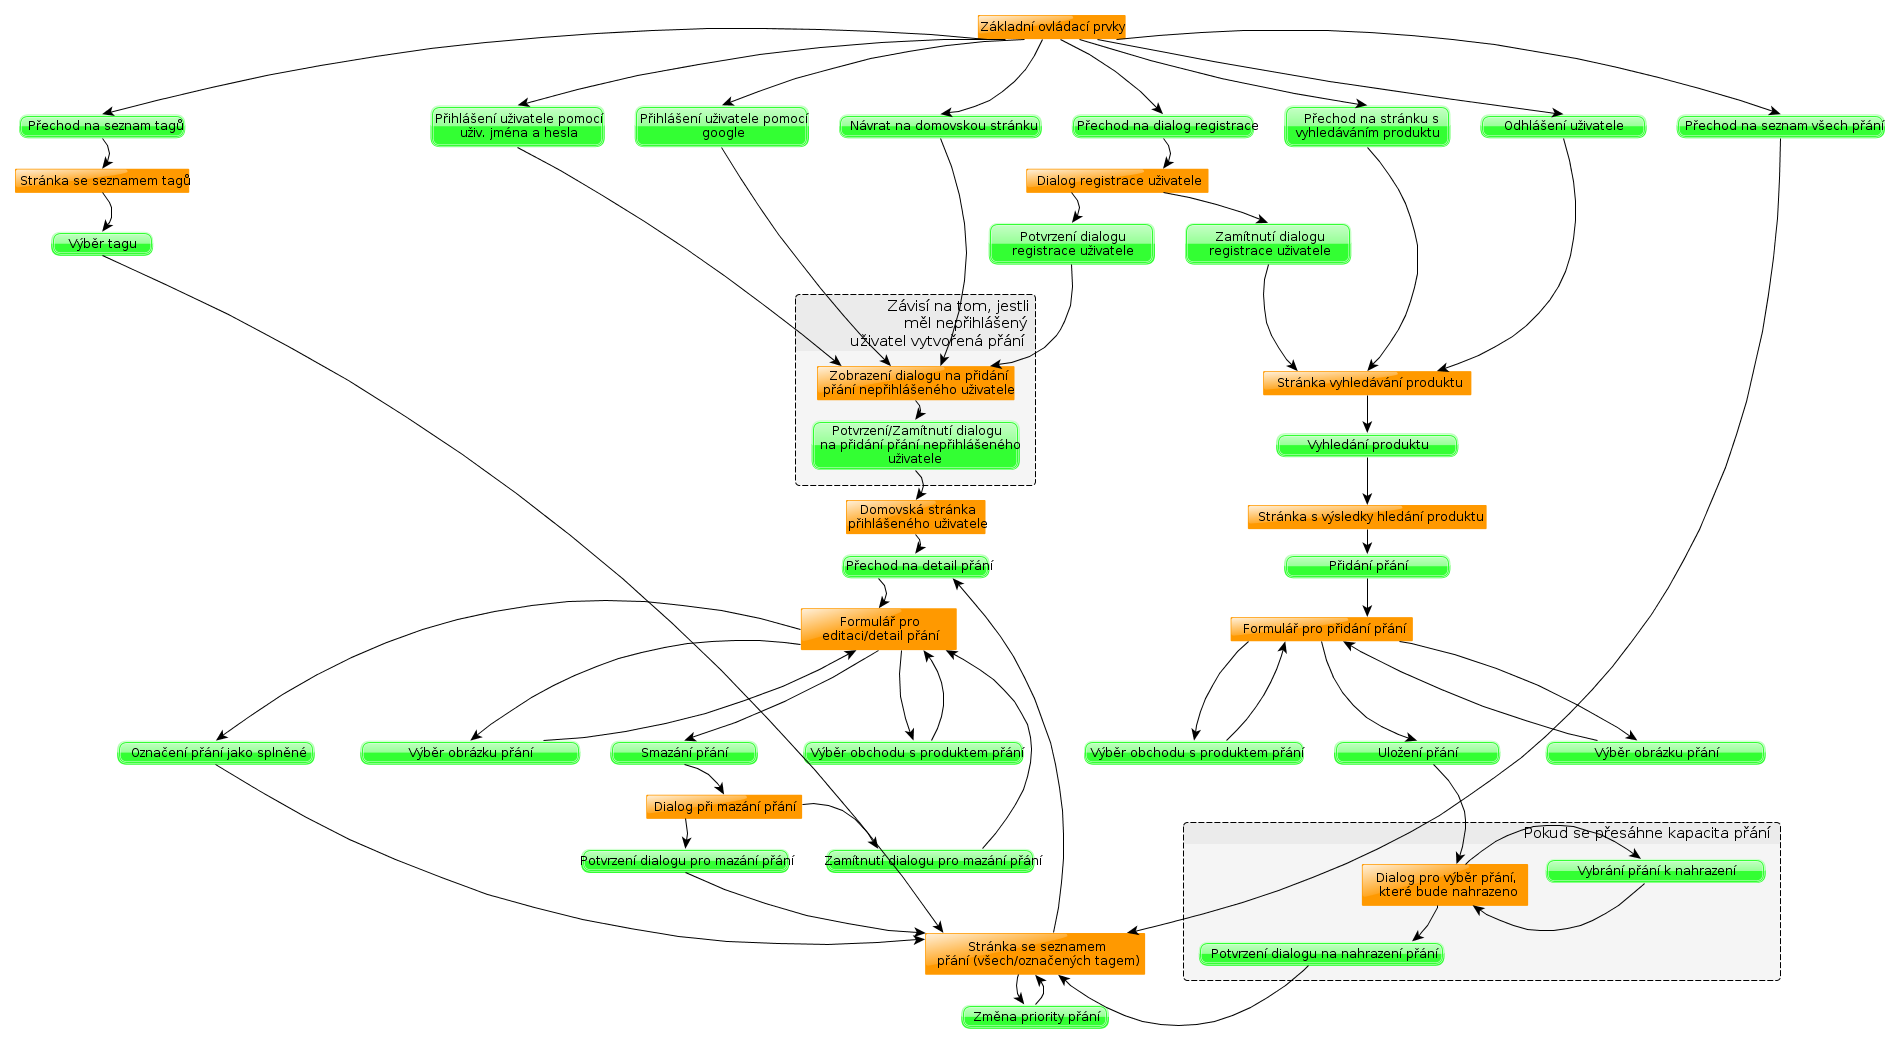
\includegraphics[width=150mm]{./pictures/taskGraph.png}
\caption{Diagram operací pro návrh GUI}
\label{fig:taskGraph}
\end{center}
\end{figure}

\subsection{Wireframe - Drátěný model}
Wireframe je množství ilustrací, které ukazují v malém, nebo velkém detailu obsah každé stránky. Typicky jsou nakresleny pomocí jednoduchých čar, není to vyčerpávající návrh vzhledu. Mimo jiné ukazují jaké informace budou dostupné na jaké stránce. Wireframe je jedním z více kontroverzních dokumentů návrhu uživatelského rozhranní, protože spojují dohromady (tedy nerozlišují mezi) strukturou informací a jejich vizuálním návrhem. Jinými slovy wireframe překračuje hranici mezi strukuturou (jaké mají mezi sebou různé infomrace vztah) a vzheldem (jak budou informace prezentovány na obrazovce)\cite{brown2007communicating}.

Kompletní návrh je včetně obrázků v příloze \ref{chp:wireframe}. Proto v této části práce budou pouze stručně popsány nejdůležitější body.

\subsubsection{Využití Nielsenovy heuristiky při návrhu}
Při návrhu obrazovek bylo postupováno podle všech pravidel heuristiky pro vyhodnocení uživatelských rozhranní popsané Jakobem Nielsenem\cite{molich1990improving}. Konkrétně:
\begin{enumerate}
\item \textbf{viditelnost stavu systému} - název stránky umístěný v horní části stránky
\item \textbf{shoda systému a reálného světa} - veškeré názvosloví v aplikaci např. štítky a přání, ovládací prvky na obrazovkách jsou sobrazeny v logickém pořadí, tedy důležitější nahoře, nebo vlevo
\item \textbf{svobodné akce uživatele} - aplikace vždy umožňuje pomocí zpět přejít na předchozí stránku, odkaz na domovskou stránku je vždy dobře dostupný (dvakrát umístěn v layoutu stránky)
\item \textbf{konzistence a standardy} - hlavní menu je v levém panelu, název stránky odkazuje na hlavní stranu
\item \textbf{prevence chyb} - použití JavaScript validací, které uživatele informují o chybě ještě než ji odešle na server. Minimalizace textových vstupních polí pro uživatele
\item \textbf{preference rozpoznání před vzpomínáním} - všechny důležité informace jsou uživateli zobrazeny na obrazovce se kterou právě pracuje. Např. v obrazovce \ref{sc-10} jsou uživateli všechna přání vyčtena, místo toho aby si musel pamatovat, která přání jako nepřihlášený uživatel vytvořil.
\item \textbf{flexibilita a efektivnost použití} - Nepřihlášenému uživateli se zobrazuje nápověda u hlavních ovládacích prvků, zatímco přihlášenému (tedy zkušenému) nikoli. Systém je celkově velmi jednoduchý, žádné zkratky v něm nebyly navrženy.
\item \textbf{efektivní informační design} - množství zobrazených informací bylo pro přehlednost minimalizováno. U přání se vývoj ceny zobrazuje pomocí grafu.
\item \textbf{pomoc při rozpoznávání, stanovení chyb a následné zotavení} - chybové zprávy byly navrženy s ohledem na toto pravidlo
\item \textbf{nápověda a dokumentace orientovaná na úkoly} - Systém obsahuje pouze minimální nápovědu poskytnutou formou popup oken\footnote{JavaScriptová okénka, která se zobrazí pokud uživatel najede myší nad daný prvek} nad hlavními ovládacími prvky.
\end{enumerate}

\section{Návrh implementace}
Přestože je implementace výsledné aplikace daná vybranou technologí, existuje několik částí, které jsou spíše algoritmické a použitá technologie na ně nemá velký vliv. Přesně tyto části aplikace budou rozebrány v této kapitole.

\subsection{Algoritmus pro vytvoření spojového seznamu v databázi}
Běžný způsob jak uložit data v moderních aplikacích je uchování v relačních databázích. Takovým způsobem budou uložena i jednotlivá přání ve výsledné aplikaci.

Každé přání ma prioritu. Tato priorita je v podstatě odkazem na umístění přání v seznamu všech přání. Mějme tři přání, jedno má vysokou, druhé střední a třet nízkou prioritu. Vysoká priorita prvního přání je informace o tom, že přání má být umístěno na prvním místě v seznamu. Střední priorita je informace o tom že se přání nachází v seznamu uprostřed atd.

Reprezentace této informace v databázi může být realizována dvojím způsobem, který zároveň určuje algoritmus pro ukládání/získávání přání.

\subsubsection{Priorita jako celé číslo}
Do tabulky přání je možné vložit jeden sloupec s celočíselným datovým typem nazvaný např. \verb|priorita|. Poté se určí jestli vyšší hodnota tohoto sloupce znamená nižší, nebo vyšší prioritu.
\begin{table}
	\begin{center}
	  \begin{tabular}{ | l | c | }
	    \hline
	    NÁZEV & PRIORITA  \\ \hline \hline
	    přání1 & 1  \\ \hline
	    přání2 & 2 \\ \hline
	     &  \\ \hline
	  \end{tabular}
	  \caption{Tabulka v databázi s celočíselnou prioritou}
	  \label{tab:integer-priority}
	\end{center}
\end{table}


Nyní stačí vkládat do tabulky přání a nastavovat hodnotu sloupce \verb|priorita| tak, aby odpovídala chtěnému umístění přání v seznamu. Problém nastane ve chvíli, kdy máme přání1 s prioritou=1, přání2 s prioritou=2 (viz tabulka \ref{tab:integer-priority})a chceme do databáze přidat přání3, které bude mít nižší prioritu než přání1 a vyšší než přání2. V tuto chvíli nemáme žádnou celočíselnou hodnotu priority, kterou bychom mohli přání3 přidělit, abychom dostali kýžený výsledek. Jedinou možností je změnit prioritu už uložených přání tak, aby vzniklo místo pro přání nové.

V tomto příkladu je úprava přání v databázi triviální, ale při větším počtu záznamů může být úprava náročná. 

\subsubsection{Priorita jako odkaz}
Do tabulky přání je možné vložit sloupec se stejným datovým typem jaký má primární klíč v této tabulce a nazvat ho např \verb|NEXT_INDEX|. Tento sloupec bude odkazovat vždy na přání s nížší prioritou.

Narozdíl od metody s celočíselnou prioritou zde nenastává při vkládání nového záznamu žádný problém. Pokud chci vložit nové přání3 mezi přání1 a přání2, nastavím u přání1 jako následovníka přání3 a u přání3 nastavím jako následovníka přání2.

Problém u této metody záznamu přichází ve chvíli, kdy chceme dostat přání z databáze seřazené podle priority.

\subsection{Algoritmus určení počáteční priority přání}
% !TEX root = ../DP_Vik_Tomas_2013.tex
\chapter{Implementace}
Pro lepší představu bude nejdříve zběžně popsán způsob, jakým se všeobecně sestavuje aplikace ve frameworku Ruby on Rails. Následně se bude kapitola věnovat detailněji implementaci napojení aplikace na srovnávač Heureka.cz, implementací získávání aktuálních cen a jejich zpracování do grafu a kapitolu uzavře ukázka implementovaných obrazovek aplikace.

\section{Standardní rozvržení aplikace v Ruby on Rails}
Jak již bylo řečeno v kapitole \ref{sec:ror}, aplikace upřednostňuje konvenci před konfiguraci, což na jednu stranu znamená minimum konfigurace aplikace, na druhou stranu to znamená, že má vývojář přesně dané postupy jak v implementaci něčeho dosáhnout. Framework je postaven na návrhovém vzoru MVC a to také implementaci rozděluje na tři významné části.

\subsection{Model}
Model reprezentuje informace v aplikaci a pravidla jak s nimi zacházet. Což se dá interpretovat také jako mechanismus zapisování a čtení databáze a pravidla tohoto zápisu/čtení. Model je v Rails řešen pomocí knihovny Active Record. Ta poskytuje nad každým objektem modelu velkou škálu funkcí které manipulují přímo s databází. Každá modelová třída musí dědit od |ActiveRecord::Base|. Na schématu \ref{fig:model-diagram} jsou vidět všechny modelové třídy ve výsledné aplikaci. Každý model v Rails má v příslušné tabulce v databázi ještě dva sloupce |create_at| a |updated_at| jejichž hodnoty se automaticky nastavují při vytvoření/upravení záznamu.

\begin{figure}[htb]
\begin{center}
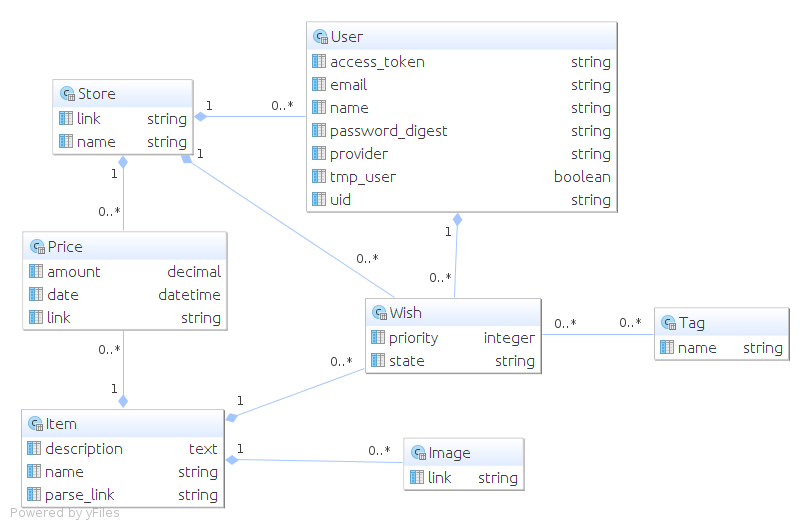
\includegraphics[width=120mm]{./pictures/model-diagram.png}
\caption{Diagram tříd v modelu aplikace}
\label{fig:model-diagram}
\end{center}
\end{figure}

\subsection{Controller}
Controller je v Rails třída, která dědí od třídy |ActionController::Base|. Tato třída má na starosti zpracování HTTP dotazů. Pokud přijde dotaz, framework se pokusí v routes souboru\footnote{Konfigurační soubor, ve kterém jsou nastaveny pro každou validní URL odpovídající controllery a jejich metody.} najít vhodný controller a jeho metodu, kterou poté zavolá. Controller má mimo jiné přístup k parametrům, se kterými byl proveden HTTP dotaz a k session proměnné.

Dále je v Rails aplikacích standardem, že existuje controller, který se nazývá |ApplicationController| a od něj dědí všechny ostatní controllery. Tak je tomu i ve výsledné aplikaci.

V následující ukázce je kus kódu největšího controlleru výsledné aplikace |WishesController|. Konkrétně metoda, která se volá po odeslání formuláře na přidání přání.

\lstset{language = ruby, style=custom}
\begin{lstlisting}
class WishesController < ApplicationController

#....... kod vynechan

  # POST /wishes
  # POST /wishes.json
  def create
    #ziskame prani pro id z parametru
    @wish = Wish.new(params[:wish])
    #z retezce ziskame stitky
    tags = Tag.parse_tags(params[:tags])
    @wish.tags = tags
    @wish.user = current_user
    #inicializujeme prioritu prani
    @wish.initialize_priority(params[:user_priority].to_d)
    respond_to do |format|
      format.html { redirect_to wishes_path, notice: :success }
      format.json { render json: @wish, status: :created, location: @wish }
    end
  end

#....... kod vynechan

end
\end{lstlisting}

\subsection{View}
View reprezentuje uživatelské rozhraní aplikace. V Rails je view řešeno pomocí HTML souborů, do kterých jsou vloženy kusy Ruby kódu. View poskytují data klientskému prohlížeči.

View je vykreslován controllerem a má také k dispozici všechna data, která má k dispozici controller. Proto je snadné předávat do view data získaná v controlleru.

Následuje ukázka kódu view, který má ve výsledné aplikaci na starost vykreslení seznamu štítků v levém panelu.

\lstset{language = html, style=custom}
\begin{lstlisting}
<div id="tag-overview" class="sidebar-nav">
  <div class="well">
    <ul class="nav nav-stacked nav-pills">
      <li class="nav-header">Stitky</li>
      <% @main_page_tags.each_with_index do |tag, index| %>
          <li <%= 'class=overflow' if index > 4  %>>
            <a href="/wishes/bytag/<%= tag.name %>">
              <%= truncate(tag.name, length: 12) %> <%= raw(ApplicationHelper.badge(tag.wish_count(current_user.id))) %>
            </a>
          </li>

      <% end %>
      <% if @main_page_tags.size > 4 %>
          <li><a id="more-tags-button" class="more" href="#"><i class="icon-chevron-down"></i>Vice</a></li>
      <% end %>
    </ul>
  </div>
</div>
\end{lstlisting}

\section{Napojení výsledné aplikace na srovnávač Herueka.cz}
Jako zdroj dat pro aplikaci je využit server pro srovnávání cen \textbf{Heureka.cz} a způsob získávání dat z tohoto serveru je \textbf{Web scraping}. Pro usnadnění získávání dat z webových stránek je použita knihovna Nokogiri\footnote{\url{http://nokogiri.org/}}.

Získávání dat spočívá v dotazování na specifické URL serveru. To má vždy stejnou podobu, například získání dokumentu s výsledky hledání produktu vypadá následovně:

\lstset{language = ruby, style=custom}
\begin{lstlisting}
doc = Nokogiri::HTML(open("http://www.heureka.cz/?h[fraze]=#{heureka_term}"))
\end{lstlisting}

\noindent kde |heureka_term| je vyhledávaný výraz.

V takto získaném dokumentu je snadné hledat jednotlivé elementy pomocí CSS selektorů (viz. \ref{sec:css-selektor}) a číst obsah takto získaných elementů pomocí metody. Následuje ukázka kódu\footnote{Pro přehlednost bylo z ukázky odebráno přiřazení získaných dat.} na získání produktů z vyhledávání provedeného předchozím příkazem:

\begin{lstlisting}
products = doc.css('#content #search .product')
products.each do |product|
  image_link = product.css('.foto img').first['src']
  description_document = product.css('.desc p.small').first
  if description_document
    search_item.description = description_document.content
  end
  item_link = product.css('div h2 a').first
  #nazev produktu
  name = item_link.content
  #odkaz na tento produkt, ze ktereho se prani ziska
  parse_link = item_link['href']
  #pokud odkaz nevede na heureku => neslo by parsovat dalsi data
  next if search_item.parse_link.include? 'exit'
  price_from_to = product.css('.wherebuy .price a.pricen').first.content
  price_from = price_from_to.split('-').first.gsub(/[^0-9]/i, '')
  price_to = price_from_to.split('-').last.gsub(/[^0-9]/i, '')
end
\end{lstlisting}

Základními metodami naimplementované knihovny pro získávání dat ze serveru Heureka.cz jsou:

\begin{itemize}
\item |search_term(term, limit)| - vrátí vyhledané produkty, tyto produkty nejsou ještě vloženy do databáze, každý vyhledaný produkt obsahuje URL, ze kterého je možné jeho data získat
\item |parse_item(item_url)| - je volána při přidávání přání s novým produktem, získá z dané URL produkt, uloží všechny jeho informace do databáze a vrátí jej
\item |get_prices(item)| - volá se při vytváření nového přání a poté periodicky každý den. Získá ceny ze všech obchodů, ve kterých se produkt z~parametru prodává.
\end{itemize}

Při implementaci získávání dat metodou Web Scraping bylo nejobtížnější ošetřit všechny možné podoby stránek, které server vrací. Např. videa v galerii obrázků, žádný popis nebo obrázek produktu apod.

\section{Získávání cen a sestavování grafu vývoje ceny}

\section{Výsledné grafické uživatelské rozhraní.}

% !TEX root = ../DP_Vik_Tomas_2013.tex
\chapter{Vyhodnocení}
Výsledná aplikace má model otestovaný pomocí unit testů. Ty ověřují základní funkčnost algoritmů a metod pro práci s daty modelu. Funkční a integrační testy v aplikaci přítomny nejsou.

Při vývoji aplikace byl kladen důraz na návrh uživatelského rozhraní a tento návrh je také potřeba důkladně vyhodnotit.

Důvod proč vyhodnotit návrh UI je zřejmý, výsledná aplikace má uživatelské rozhraní, které vývojář podle všech dostupných informací navrhnul tak, aby bylo jednoduché na používání (viz. kapitola \ref{sec:navrh-gui}). Na konci vývojového cyklu je třeba ověřit, že úsudky v návrhu byly správné.  

Během celého procesu vývoje práce byl návrh konzultován s možnými uživateli a na základě těchto konzultací a připomínek při nich získaných byl návrh upraven do finální podoby popsané v příloze \ref{chp:wireframe}.

\section{Způsoby vyhodnocení návrhu uživatelského rozhraní}
Základem vyhodnocení je uživatel a jeho práce se systémem. V této části práce budou popsány některé metody, které se používají pro zaznamenání činnosti uživatele, resp. pro zaznamenání okamžiků, nebo situací kdy uživatel nejednal předpokládaným způsobem. Například se v nějakém kroku od uživatele může čekat, že zadá vstup a on se místo toho pokusí odeslat formulář atp.

\subsection{Osobní konzultace}
Hlavně v raných stádiích vývoje je nejlepší osobní kontakt s uživatelem\cite{stone2005user}. Je mnoho variací jak zvýšit efektivitu osobní konzultace.

Například je možné podporovat uživatele v tom, aby "přemýšlel nahlas" a poté si všímat, kdy se uživatelovy myšlenky odchylují od očekávaných. Tento způsob testování ovšem není pro každého uživatele a někteří jej mohou shledat rušivým a zároveň tento způsob testování nutí uživatele více přemýšlet a provádět kroky v aplikaci pomaleji (protože zároveň sděluje své myšlenky) a to může způsobit, že uživatel neudělá chyby, které by normálně udělal.\cite{stone2005user}.

Nejvíce zpětné vazby lze získat samotným pozorováním uživatele bez toho, aby mu byla poskytnuta jakákoli pomoc při ovládání aplikace. Je možné se uživatele zeptat na otázky jako: "Co se snažíte udělat?", nebo "Co jste čekal, že se stane, když jste kliknul na to tlačítko?", ale je těžké najít správný poměr otázek tak, aby se příliš nerušila uživatelova pozornost\cite{stone2005user}.

\subsection{Sezení s audiovizuálním záznamem}
Audiovizuální záznam sezení může pomoci zaznamenat přesná místa, ve kterých se uživatel dostal do problémů a zároveň slouží jako záloha pozorování, pokud by pozorovateli cokoli uniklo. Pokud se na projektu podílí více lidí, může být záznam sezení brán například jako důkaz závažnosti problému v návrhu aplikace.\cite{stone2005user}

Na obrázku \ref{fig:testing-camera} je vidět správné umístění kamery, která zabírá zároveň uživatele a zároveň obrazovku na které je zrcadlena uživatelova plocha. Tak je možné sledovat uživatele i jeho akce.\cite{stone2005user}

\begin{figure}[htb]
\begin{center}
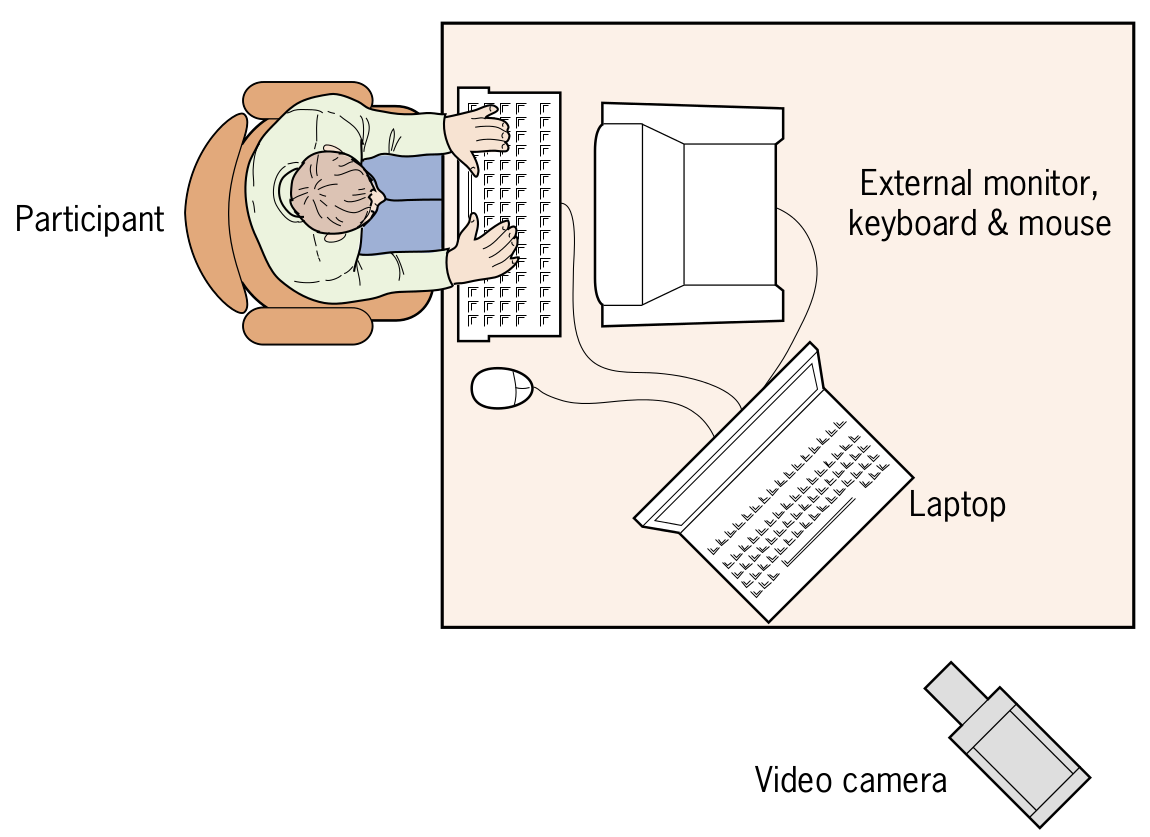
\includegraphics[width=100mm]{./pictures/testing-camera.png}
\caption{Schéma správného umístění kamery k počítači a respondentovi\cite{stone2005user}}
\label{fig:testing-camera}
\end{center}
\end{figure}

\subsection{Sledování pohybu očí}
Metoda přesného snímání pohybu očí respondenta může odhalit chování, které nelze postřehnout ostatními metodami. Díky tomuto sledování je možné zjistit, na které části obrazovky se respondent kouká a kdy se na ně kouká. Pomocí zpracování takových dat od více respondentů je možné zjistit, jaká místa na obrazovce jsou jak prohlížena a tomu přizpůsobit rozmístění ovládacích prvků. Moderní zařízení pro pořízení tohoto záznamu vypadají velmi podobně jako obyčejný monitor, nebo jsou dodávána v podobě malého přídavného zařízení pod monitor (obrázek \ref{fig:tobii}).

\begin{figure}[htb]
\begin{center}
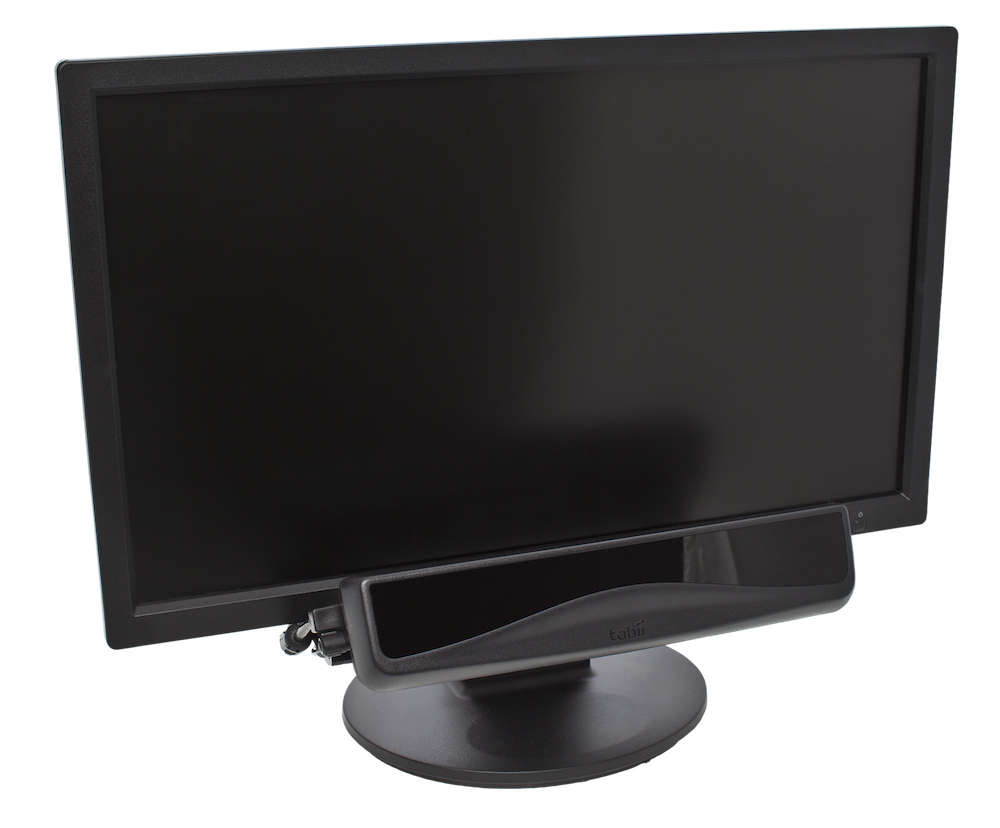
\includegraphics[width=60mm]{./pictures/tobii_image_pceye_mounted_front_rgb.jpg}
\caption{Přídavné zařízení Tobii PCEye pro sledování pohybu očí}
\label{fig:tobii}
\end{center}
\end{figure}

\subsection{Záznam akcí}
Pokud je důležité, jak rychle trvá uživateli vykonat akce v aplikaci, tedy každý klik a každý stisk klávesy se počítá, pak je vhodné použít nástroje na zaznamenávání uživatelských akcí\cite{stone2005user}. Tyto nástroje vychází ze tří základních druhů produktů\cite{stone2005user}:
\begin{itemize}
\item Produkty sledující že uživatel dělá svojí práci a nesnaží se narušit bezpečnost systému
\item Produkty, které nahrávají uživatelské akce za účelem pozdější prezentace této akce
\item Webové produkty, které získávají informace o uživatelově pohybu mezi stránkami a četnosti návštěv.
\end{itemize}

\subsection{Dotazník}
Dotazník je jednoduchá forma získání respondentova názoru pomocí tištěné nebo elektronické verze dokumentu, ve kterém jsou otázky na témata týkající se testovaného subjektu. Otázky mohou být uzavřené, kdy uživatel může zvolit jednu z předem daných možností, nebo otevřené, kdy má uživatel možnost rozvést odpověď vlastním textem.

Použití dotazníku při vyhodnocení má mnohé výhody\cite{stone2005user}:
\begin{itemize}
\item Všechny otázky jsou napsány, na žádnou se nezapomene.
\item Všichni účastníci dostanou stejnou otázku, a proto je možné mezi sebou porovnávat odpovědi.
\item Dají se pomocí něj získat kvantitativní data jako: 10 uživatelů považovalo navigaci aplikací náročnou.
\end{itemize}
Zároveň má použití dotazníku několik nevýhod\cite{stone2005user}:
\begin{itemize}
\item Je těžké dotazník navrhnout tak, aby mohl být jedinou metodou vyhodnocení. Otázky mohou zavádět, nebo nemusí mít v nabídce odpověď, která by uživateli vyhovovala.
\item Musí se předem odhadnout témata, o kterých uživatel bude chtít po testování aplikace mluvit.
\item Uzavřené otázky typu: \emph{Hodnoťte na stupnici od jedné do pěti jak jednoduchá pro vás byla navigace aplikací} jsou snadné na analyzování, ale nezjistí, proč se tak uživatel cítil.
\end{itemize}

Při tvorbě dotazníku je rozumné nejprve probrat s potencionálním respondentem témata, které ho při práci s aplikací napadnou a ta do dotazníku zapracovat\cite{stone2005user}.

Existuje již mnoho předpřipravených dotazníků s vypracovanými metodikami vyhodnocení. Je silně doporučeno nějaký takový dotazník použít, nebo se jím minimálně nechat inspirovat\cite{stone2005user}.

\section{Popis metodiky zvolené pro tuto práci}
\label{sec:metodika-dotaznik}
Pro vyhodnocení návrhu uživatelského rozhraní v této práci bude použit dotazník. S potencionálními uživateli byl návrh konzultován průběžně a na závěrečné vyhodnocení byl zvolen dotazník pro snadnou kvantifikaci výsledků. Dotazník se skládá ze dvou částí.

První a povinnou částí je SUS dotazník. Ten vyšel nejlépe v porovnání 5 volně dostupných dotazníků, kterou v roce 2004 prováděli Thomas S. Tullis a Jacqueline N. Stetson\cite{tullis2004comparison}. Jedná se o dotazník s deseti otázkami na které uživatel dává odpovědi v rozsahu 1-plně souhlasím až 5-vůbec nesouhlasím.

Druhou částí dotazníku jsou nepovinné otázky na funkčnost z kapitoly \ref{sec:navrh-funkcionality}. Otázky jsou zaměřeny na jednotlivé funkčnosti a jejich správné a jednoduché použití uživatelem. Pro jasnou kvantifikaci byly kromě závěrečných připomínek voleny uzavřené otázky.


\section{Vyhodnocení dotazníku}
\label{sec:vyhodnoceni-dotazniku}
Kompletní výsledky navrhnutého dotazníku jsou v příloze \ref{chp:vysledky}. Nyní budou pouze shrnuty dopady, které průzkum přinesl.

Na dotazník odpovědělo 22 respondentů. Jednalo se převážně o cílovou skupinu, tedy mladé lidi ve věkovém rozmezí 20 až 30 let.

\subsection{SUS dotazník}
Část dotazníku na kterou odpovídali povině všichni respondenti. Aplikace dosáhla u respondentů celkového skóre \textbf{79,09}, což je přesně na pomezí ohodnocení dobrý a vynikající\cite{bangor2009determining}. Což jsou druhé a třetí nejlepší ohodnocení na 7 stupňové škále, která vznikla sběrem výsledků SUS dotazníku u 250 různých aplikací\cite{bangor2009determining}.

Tento výsledek nasvědčuje tomu, že uživatelské rozhraní je pro uživatele snadno použitelné.

\subsection{Dotazník zaměřený na funkcionalitu}
Další otázky v dotazníku byly zaměřené na konkrétní funkcionalitu a zde budou interpretovány výsledky jednotlivých otázek.

Docela velké procento (24\%) respondentů si nebylo jisto, k čemu aplikace přesně slouží. Pro to existují 2 vysvětlení:
\begin{itemize}
\item Úvodní stránka aplikace dostatečně nevysvětluje k čemu aplikace slouží, nebo ji uživatelé okamžitě přeskočí.
\item Aplikace dostatečně neprezentuje svoji přidanou hodnotu svým uživateslkým rozhraním.
\end{itemize}

Pro několik respondentů bylo spíše těžké vyhledat předmět přání. Z námětů, které vzešly z dotazníku vyplynulo, že vyhledávání by měl být také hlavní ovládací prvek (nyní je to pouze tlačítko pro přechod na vyhledávání a tedy o krok více).

Naprostá většína respondentů se nepřihlásila do aplikace. To je ale pochopitelné vzhledem k tomu, že respondenti měli za úkol s aplikací pracovat pouze 10 minut a aplikace poskytuje veškerou funkcionalitu i nepřihlášenému uživateli. 18\% respondentů nevědělo, že se do aplikace lze přihlásit.

23\% respondentů v dotazkníku odpovědělo, že nepřidali žádné přání do svého seznamu. Tuto odpověď by bylo vhodné prozkoumat dalším, cíleným, dotazníkem. Může se jednat o špatně položenou otázku, nebo o chybu v uživatelském rozhraní.

43\% respondentů nepřesunulo přání ve svém seznamu a tím mu nezměnilo prioritu. Je tedy zřejmé, že tato funkcionalita nemá dobře udělané UI. Řešením je buď statická nápověda, která na možnost přesouvání přání bude uživatele stále upozorňovat, nebo grafické znázornění možnosti přesunutí. Změna tvaru kurzoru očividně nestačí.

Štítky se naopak jeví jako dobře navržené. Jejich panelu jakožto hlavního ovládacího prvku si všimla naprostá většina respondetů a 64\% jich zároveň použilo štítky pro filtrování přání. Zároveň jen 2\% respondetnů nevěděly, že mohou přání štítkem označit.

V dotazníku byla špatně formulována otázka na přidání obrázku k přání. Bylo použito slovo vlastní obrázek, pod kterým si zřejmě většina respondetů představila upload obrázku z uživatelova počítače. Otázkou bylo myšleno změna obrázku kliknutím na jinou miniaturu ve formuláři pro přidání obrázku.

44\% respondetů nevědělo, že může vybrat vlastní obchod k přání. Znovu může jít o špatně položenou otázku. Měla by znít: Vybral jsi si obchod ve formuláři pro přidání přání?

Návrh UI pro mazání přání je navržené dobře. Jen 6\% respondentů nevědělo o této funkčnosti. Stejně je na tom také zobrazení detailu přání.

29\% procent respondentů nevědělo, že může označit přání jako splňené, což znamená, že by UI pro tuto funkcionalitu mělo být také zlepšeno, nebo minimálně doplňeno nápovědou.









% !TEX root = ../DP_Vik_Tomas_2013.tex
\chapter{Možná rozšíření práce}
Některá funkcionalita byla nad rozsah této práce, nebo její absenci objevily až závěrečné testy uživatelského rozhraní. Výčtem a krátkým popisem této funkcionality se bude zabývat tato poslední kapitola.

\section{Využití API srovnávačů}
Dalším logickým pokračováním vývoje aplikace je rozhodně napojení na API samotných srovnávačů, protože i když Web Scraping funguje, není pravděpodobně udržitelný při rozšíření uživatelské základny.

Výborná funkcionalita by mohla vzejít z napojení na více než jeden srovnávač, kdy by uživatel měl ještě kvalitnější přehled o cenách svého přání v různých obchodech. Vše je ale závislé na dohodě s konkrétními servery. Ty by pravděpodobně s takovým mesh-up nesouhlasili. Zatím mají tyto servery relativně výsadní postavení na trhu a není pravděpodobné, že by chtěli poskytnout svá data aplikaci, která by je porovnávala s konkurencí a tím jim například snížila počet prokliků.

\section{Zapojení aplikace do sociálních sítí a sdílení}
V dnešní době je většina používaných webových aplikací nějakým způsobem zapojena do sociálních sítí. Aplikace by mohla například s uživatelovým souhlasem publikovat do sociálních sítí informaci o tom že si něco přeje, nebo že si přání splnil.

Dokonce by bylo dobré, kdyby člověk svůj seznam mohl sdílet, aby např. známí věděli, co můžou uživateli koupit.

\section{Plugin do prohlížeče}
Jak bylo zmíněno v kapitole \ref{sec:amazon-wishlist-button}, Amazon Wish list má plugin, který umožňuje z jakékoli stránky přidat přání do seznamu. Tato funkcionalita by byla vhodná i pro výslednou aplikaci. Pokaždé když by se uživatel nacházel na stránce srovnávače cen, ze kterého aplikace čerpá data, mohl by uživatel jedním kliknutím přidat do svých přání právě zobrazovaný předmět.

\section{Umožnit uživateli odeslat připomínku/informaci o chybě}
Aplikace by mohla obsahovat formulář, kterým by uživatel mohl vývojáře informovat o chybě v aplikaci\footnote{Vážné chyby se zaznamenávají do aplikačního logu, to ale neznamená, že nemůže nastat nějaká chyba v logice aplikace.} a nebo připomínce k aplikaci.

\section{Komplexnější vyhledávání}
Uživateli by mohl být nabídnut ekvivalent výrobku, nebo výrobek, který hledaný termín obsahuje jen v technickém popisu a ne v názvu.

\section{Trendy přání}
Zatím není aplikace schopná získat o uživateli dostatečný počet informací, aby mu mohla fundovaně nabízet přání, která by mohl chtít. Pokud by se v budoucnu aplikace tyto informace mohla dozvědět například propojením se sociální sítí, poté by byla vhodná funkcionalita, která by uživateli nabízela přání, která mají jemu podobní uživatelé.
% !TEX root = ../DP_Vik_Tomas_2013.tex
\begin{conclusion}

Moderní webové aplikace na srovnávání a nakupování popsané v rešerši jsou pro zákazníka ohromnou úsporou času a peněz při nakupování. Výsledná aplikace se snažila stavět na přidané hodnotě těchto webových aplikací a jít ještě dále v usnadnění uživatelovi činnosti.

V práci byla nalezena funkcionalita, která je běžně poskytována současnými aplikacemi a dále bylo navrženo několik funkcí, díky kterým bude výsledný seznam přání pro uživatele užitečný.

Při návrhu uživatelského rozhranní bylo postupováno v souladu s Nielsenovou heuristikou\cite{molich1990improving}. A všeobecně byl kladen velký důraz na jednoduchost UI.

Implementace proběhla v nejmodernějších technologiích, což se příznivě podepsalo na vzhledu uživatelského rozhraní, jako například dynamické donačítání dat do stránek, mnoho javascriptových modálních oken atp. Vybraná metoda získávání dat (Web Scraping) sebou přinesla jak výhody, tak několik nevýhod a to především menší interaktivitu se zdrojem dat, kvůli snaze o malé zatěžování serveru aplikace pro srovnávání cen.

Závěrečnou zkouškou aplikace bylo uživatelské testování provedené formou dotazníku pro snadnou kvantifikaci výsledků. Z tohoto testování vyplynuly následující závěry. Aplikace má dobré až výborné uživatelské rozhranní, což bylo ověřeno pomocí SUS dotazníku. Návrh UI přesto nebyl zdaleka bezchybný, což se ukázalo v části dotazníku zaměřeném na konkrétní funkce aplikace. Pro několik funkcí bylo uživatelské rozhranní navržené nedostatečně výrazně a uživatelé tyto funkce přehlédli. Dokonce ani navržení dotazníku se neobešlo bez chyby a dvě otázky se ukázaly nešťastně zforulované.

Celkově práce splnila své zadání a poskytla jedinečný pohled na systémy srovnávání cen a funkcionalitu, kterou je možné tyto velké databáze rozšířit a obohatit tak uživatelovu zkušenost.


\end{conclusion}

\bibliographystyle{csn690}
\bibliography{DP_Vik_Tomas_2013}

\appendix

% !TEX root = ../DP_Vik_Tomas_2013.tex
\chapter{Slovník pojmů}
V příloze je vysvětleno několik zálkladních pojmů, které jsou používány v celé práci.
\section{Zboží}
Zboží je hmotný statek (přírodní nebo vyrobený), který je určen k prodeji. To znamená, že zboží za určitých podmínek změní svého majitele – vlastnictví produktu přechází z prodávajícího na kupujícího. Nejčastější podmínkou pro přechod vlastnictví je zaplacení kupní ceny.
%TODO doplnit zdroj (wiki), případně sehnat nějaký lepší
\subsection{Produkt}
Jeden konkrétní typ zboží, například Nokia 3310, nebo šampon Head\&Shoulders.
\section{Přání}
Tímto označením se v celé práci rozumí entita, která je svázaná se zbožím, konkrétním uživatelem a několika dalšími entitami. Tato entita reprezentuje uživatelův zájem o zboží.

\section{Aplikace}
Aplikační software (zkráceně aplikace) je v informatice veškeré programové vybavení počítače (tj. software), které umožňuje provádět nějakou užitečnou činnost (řešení konkrétního problému, interaktivní tvorbu uživatele – např. textový procesor apod.). Aplikace využívají pro interakci s uživatelem grafické nebo textové rozhraní, případně příkazový řádek. Mezi aplikace nepatří systémový software (jádro a další součásti operačního systému, např. služba Windows, démon).

\section{Webová aplikace}
Webová aplikace v softwarovém inženýrství je aplikace poskytovaná uživatelům z webového serveru přes počítačovou síť Internet, nebo její vnitropodnikovou obdobu (intranet). Webové aplikace jsou populární především pro všudypřítomnost webového prohlížeče jako klienta. Ten se pak nazývá tenkým klientem, neboť sám o sobě logiku aplikace nezná.

\section{Výsledná aplikace}
Výslednou aplikací je míněna webová aplikace, která je předmětem této práce. Jedná se tedy o aplikaci na organizaci nákupního seznamu.

\section{Webové technologie}
\subsection{CSS selektor}
\label{sec:css-selektor}
Selektory jsou v CSS odkazy na části HTML kódu, na které se bude kaskádový styl vztahovat. Selektory je možné hierarchicky skládat. V selektoru se mohou vyskytovat tyto prvky:
\begin{itemize}
\item Všechny HTML elementy - např. |h3|
\item Identifikátory elementů (obsah id atributu) uvozené mřížkou - např. |#identifikator-nadpisu|
\item Třídy elementů (obsah class atributu) uvozené tečkou - např. |.trida-nadpisu|
\item Pseudo třídy uvozené dvojtečkou - např. |:hover| pro styl prvku, nad kterým se nachází kurzor myši
\end{itemize}
Tyto selektory je možné libovloně kombinovat. Pokud se za sebe vloží bez mezery, musí se vztahovat na jeden element. Pokud je mezi nimi mezera, jedná se na odkaz do hierarchie.
% !TEX root = ../DP_Vik_Tomas_2013.tex
\chapter{Seznam použitých zkratek}
% \printglossaries
\begin{description}
	\item[GUI] Graphical user interface
	\item[XML] Extensible markup language
	\item[URL] Unified Resource Locator
	\item[MVC] Model View Controller
	\item[HTTP] Hyper Text Transfer Protokol
	\item[API] Application Programming Interface
	\item[URL] Uniform Resource Locator
\end{description}
% !TEX root = ../DP_Vik_Tomas_2013.tex
\chapter{Wireframe}
\label{chp:wireframe}
Díky prostorové náročnosti se kompletní dokumentace vytvoření drátěného modelu nachází zde v příloze.

\section{Hlavní ovládací prvky}
\label{sec:hlavni-ovladaci-prvky}
Hlavní ovládací prvky dokáží spouštět akce popsané v kapitole \ref{sec:hlavni-akce}. Tyto prvky musí být umístěny na každé stránce, a proto se nachází v tzv. layoutu webové aplikace. Návrh layoutu výsledné aplikace se nachází na obrázku \ref{fig:mock-layout}.

\begin{figure}[htb]
\begin{center}
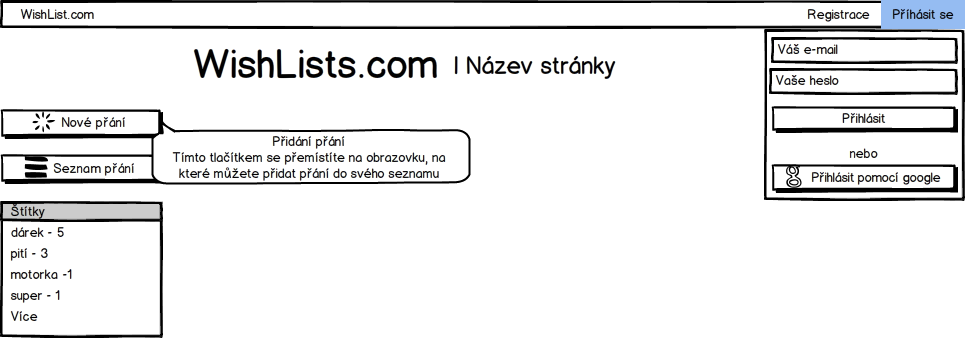
\includegraphics[width=130mm]{./pictures/mock/layout.png}
\caption{Drátěný model layoutu stránky.}
\label{fig:mock-layout}
\end{center}
\end{figure}

V návrhu layoutu je jasně vidět panel umístěný v horní časti stránky, který obsahuje prvky pro přihlášení a odkaz na domovskou stránku. Dále je v horní části stránky název aplikace, který je zároveň také odkazem na domovskou stránku. V levé části se nachází navigace, která se skládá z odkazů na přechod na přidání přání a seznam přání a ze seznamu všech štítků, u kterých je zároveň uvedeno, kolik přání je u nich obsaženo.

\section{Hlavní obrazovky}
Dále budou popsány obrazovky, které zabírají celou stránku. Tyto stránky vždy obsahují výše zmíněné \nameref{sec:hlavni-ovladaci-prvky}. Všechny obrazovky kromě \ref{sc-01} jsou navrhnuty z pohledu nepřihlášeného uživatele\footnote{Hlavní ovládací prvky umožňují přihlášení a registraci namísto odhlášení.}.

\subsection{\ref{sc-01}}
Toto je stránka, která se zobrazí uživateli ihned po jeho přihlášení do aplikace. Zároveň ho na ní přesunou oba odkazy umístěné v hlavních ovládacích prvcích. Na této stránce bude uživateli zobrazeno maximálně pět přání. Výběr přání bude proveden na základě nejprudší změny ceny (a to ať už zlevnění, nebo zdražení produktu). Stránka je na obrázku \ref{fig:uvodni-prihlaseny-uzivatel}.

\begin{figure}[htb]
\begin{center}
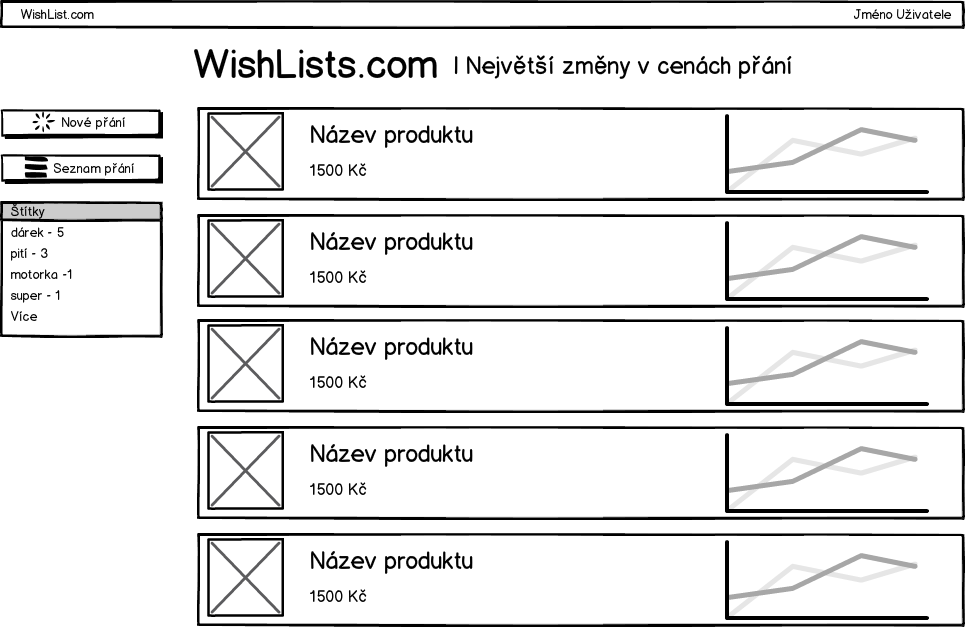
\includegraphics[width=130mm]{./pictures/mock/uvodni-prihlaseny-uzivatel.png}
\caption{\ref{sc-01}}
\label{fig:uvodni-prihlaseny-uzivatel}
\end{center}
\end{figure}

\subsection{\ref{sc-02}}
Na tuto stránku uživatel přejde, pokud zvolí hlavní ovládací prvek přidat přání. Zde je uživateli umožněno vyhledat produkt podle jeho názvu. Návrh je na obrázku \ref{fig:vyhledavani}. V centru stránky je velké vstupní pole pro zadání názvu produktu.

\begin{figure}[htb]
\begin{center}
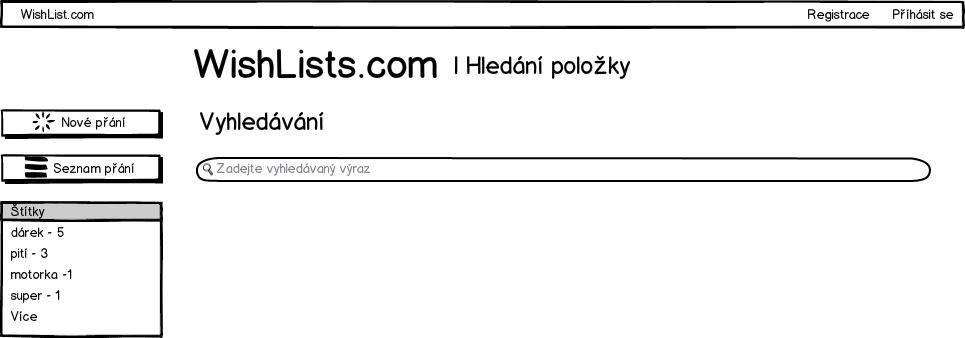
\includegraphics[width=130mm]{./pictures/mock/vyhledavani.png}
\caption{\ref{sc-02}}
\label{fig:vyhledavani}
\end{center}
\end{figure}

\subsection{\ref{sc-03}}
Po zadání hledaného výrazu zobrazí aplikace uživateli výsledky. Pokud nenajde žádný výsledek, zobrazí zprávu, která o tom uživatele informuje. Návrh obrazovky je na obrázku \ref{fig:vysledky-hledani}

U každého výsledku je ukázán obrázek produktu, jeho celý název, popisek, rozmezí cen, ve kterém se produkt pohybuje a tlačítko pro vytvoření přání. Ve skutečnosti celý výsledek reaguje na kliknutí myši. Tlačítko je u výsledku primárně, aby uživatel věděl, co se s výsledkem dělá.

\begin{figure}[htb]
\begin{center}
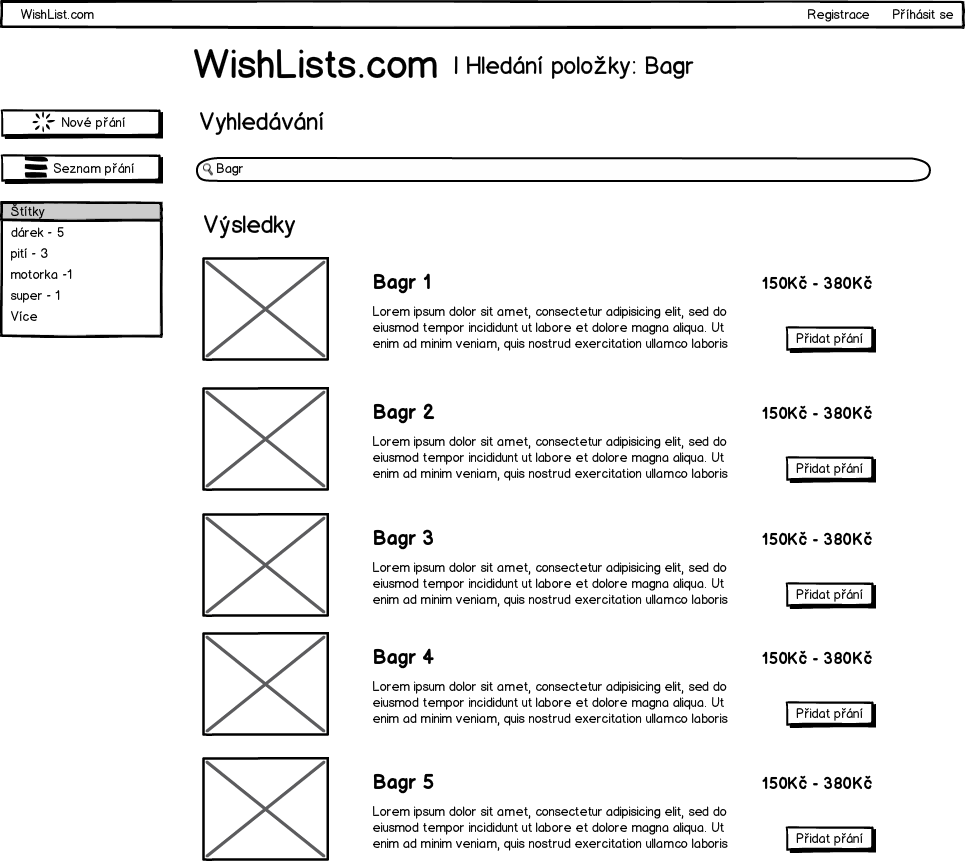
\includegraphics[width=130mm]{./pictures/mock/vysledky-hledani.png}
\caption{\ref{sc-03}}
\label{fig:vysledky-hledani}
\end{center}
\end{figure}

\subsection{\ref{sc-11}}
\label{sec:wireframe-pridani-prani}
Poté co uživatel klikne na výsledek hledání přání, bude zobrazena obrazovka pro přidání přání.  Návrh obrazovky je na obrázku \ref{fig:formular-pridani-prani}.

Na návrhu je vidět, že uživateli je zvolen obrázek pro přání, ale zároveň má možnost vybrat z miniatur pod hlavním obrázkem a kliknutím na miniauturu nahradit původní obrázek. Vizuální stránka přání je důležitá, proto zabírá celou půlku formuláře. V druhé půlce je uživateli umožněno nastavit všechny informace popsané v kapitole \ref{sec:pridani-prani}.

Rychlá priorita ulehčuje uživateli práci. Oprosťuje uživatele od vnitřní datové reprezentace priority. Nechá ho vybrat ze tří možností a na základě jednoduchého algoritmu patřičně přiřadí prioritu k přání.

Uživateli se navíc zobrazí dodatečné informace (popis a technická specifikace) o produktu, aby se mohl rozhodnout, jestli je produkt opravdu to, co hledal.

\begin{figure}[htb]
\begin{center}
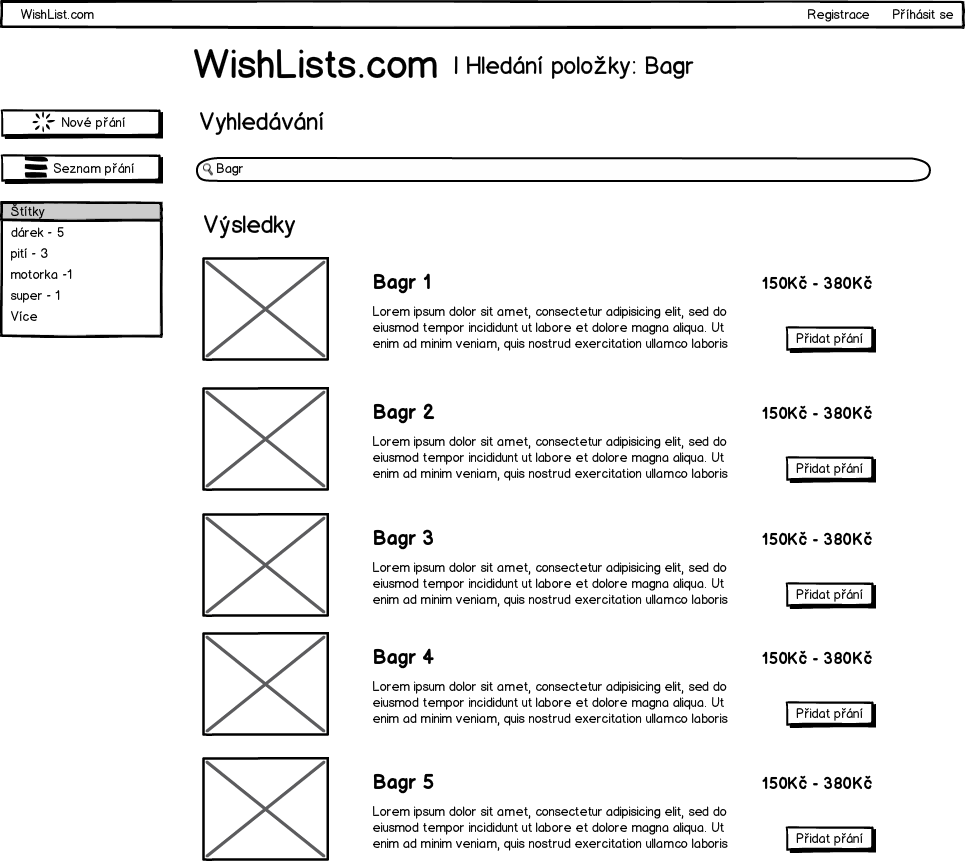
\includegraphics[width=130mm]{./pictures/mock/vysledky-hledani.png}
\caption{\ref{sc-11}}
\label{fig:formular-pridani-prani}
\end{center}
\end{figure}

\subsection{\ref{sc-04}}
Na stránce jsou uživateli zobrazena všechna jeho přání seřazena podle priority od nejvyšší po nejnižší. Návrh obrazovky je na obrázku \ref{fig:vsechna-prani}.

U každého přání je zobrazen název produktu, cena v obchodě, který je u přání přiřazen a graf aktuálního vývoje ceny.

Přání je možné přesouvat táhnutím myši a tím měnit jejich prioritu.

\begin{figure}[htb]
\begin{center}
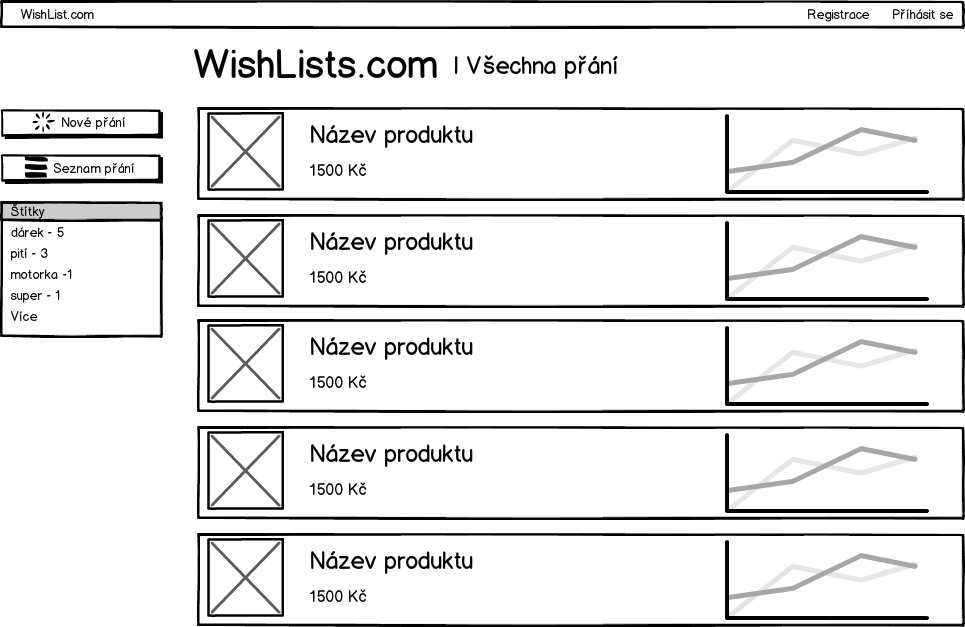
\includegraphics[width=130mm]{./pictures/mock/vsechna-prani.png}
\caption{\ref{sc-04}}
\label{fig:vsechna-prani}
\end{center}
\end{figure}

\subsection{\ref{sc-05}}
Stránka zobrazení detailu přání s možností jeho editace. Při návrhu stránky byl kladen důraz na co největší podobu se stránkou na přidání přání. Tu se totiž už uživatel musel naučit/pochopit, a proto by bylo kontraproduktivní jej nutit přemýšlet nad jinou stránkou. To odpovídá principu konzistence a standardizace\cite{molich1990improving}. Návrh obrazovky je na obrázku \ref{fig:editace-detail-prani}.

Oproti obrazovce na přidání přání byla odstraněna rychlá priorita, protože ta se teď už nastavuje na obrazovkách se seznamy přání. Přibylo tlačítko na smzání přání a důležité tlačítko, které přání označí jako splněné.

\begin{figure}[htb]
\begin{center}
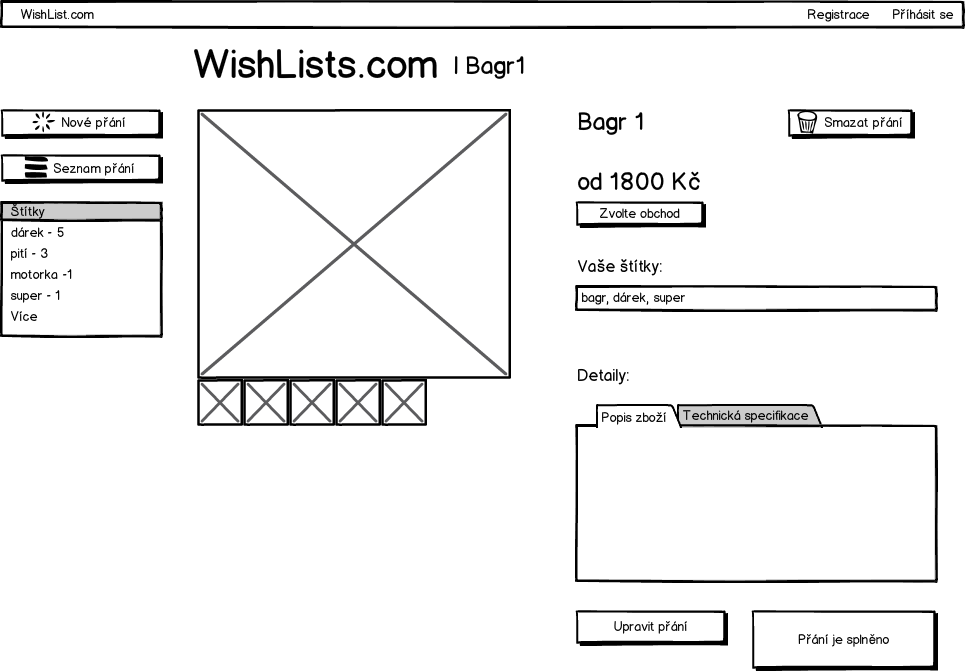
\includegraphics[width=130mm]{./pictures/mock/editace-detail-prani.png}
\caption{\ref{sc-05}}
\label{fig:editace-detail-prani}
\end{center}
\end{figure}

\subsection{\ref{sc-08}}
\label{sec:prani-podle-stitku}
Obrazovka je totožná s \ref{sc-04}, s výjimkou že jsou na ní zobrazeny pouze přání označená jedním konkrétním štítkem. Veškeré ostatní informace a funkcionalita stránky zůstavají nezměněny. Návrh obrazovky je na obrázku \ref{fig:prani-oznacena-tagem}.

\begin{figure}[htb]
\begin{center}
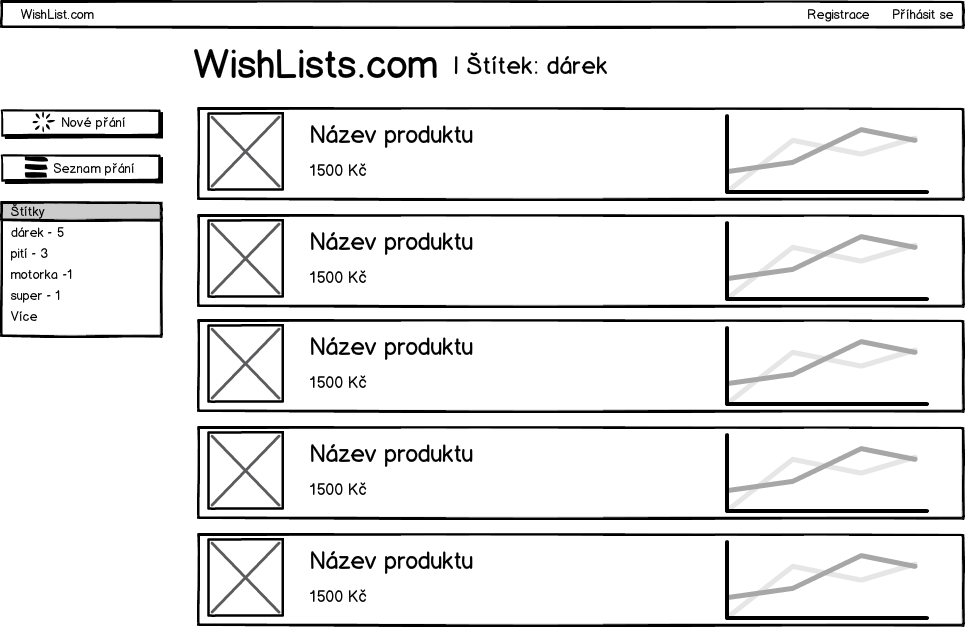
\includegraphics[width=130mm]{./pictures/mock/prani-oznacena-tagem.png}
\caption{\ref{sc-08}}
\label{fig:prani-oznacena-tagem}
\end{center}
\end{figure}

\section{Dialogy a komponenty}
Některé informace nevyžadují tolik místa, nebo je podle konvence nutné je řešit dialogem(konzistence a standardizace\cite{molich1990improving}), a proto není jejich zobrazení realizováno jako celá stránka. Namísto toho je informace zobrazená formou komponenty umístěné na hlavní ztránce, nebo dialogu zobrazeného přes libovolnou stránku.

\subsection{\ref{sc-12}}

\subsection{\ref{sc-06}}
Na obrázku \ref{fig:dialog-mazani-prani} je zobrazen návrh dialogu, který se uživateli zobrazí poté, co klikne na tlačítko smazání přání. Dialog je naprosto triviální.

\begin{figure}[htb]
\begin{center}

\includegraphics[width=70mm]{./pictures/mock/dialog-mazani-prani.png}
\caption{\ref{sc-08}}
\label{fig:dialog-mazani-prani}
\end{center}
\end{figure}

\subsection{\ref{sc-07}}
Komponenta je přítomna v základním layoutu a je vidět například na obrázku \ref{fig:mock-layout}. Jedná se o seznam všech štítků, kterými má uživatel označena přání. Skládá se z nadpisu komponenty, seznamu štítků a tlačítka, které umožňuje zobrazovat/skrývat další štítky. Každý šítek má u sebe zobrazeno číslo reprezentující počet přání, které jsou jím označeny. Zároveň štítek funguje jako odkaz na obrazovku s přehledem štítků (\ref{sec:prani-podle-stitku}).

Po zobrazení komponenty se v ní pro přehlednost ukazuje pouze pět nejpoužívanějších štítků. Další může uživatel zobrazit pomocí stisknutí tlačítka \emph{Více}.

\subsection{\ref{sc-09}}
Na obrázku \ref{fig:dialog-registrace} je zobrazen návrh formuláře pro registraci uživatele. Tento formulář je zobrazen v dialogu. Uživatel na něm vyplní pouze nezbytné údaje pro správnou registraci:
\begin{itemize}
\item Celé své jméno
\item E-mail
\item Heslo pro přihlášení
\end{itemize} 

\begin{figure}[htb]
\begin{center}
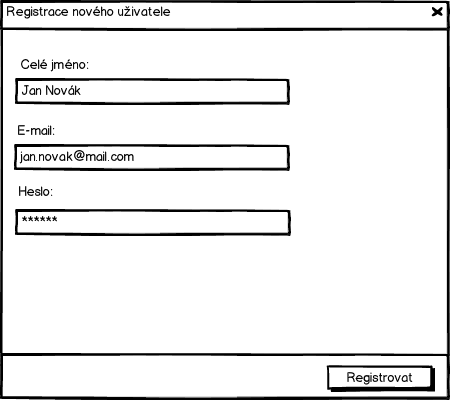
\includegraphics[width=70mm]{./pictures/mock/dialog-registrace.png}
\caption{\ref{sc-09}}
\label{fig:dialog-registrace}
\end{center}
\end{figure}

\subsection{\ref{sc-10}}
Na obrázku \ref{fig:dialog-pridani-docasnych-prani} je zobrazen návrh dialogu, na kterém má uživatel těsně po přihlášení možnost přidat ke svým přáním ta přání, která vytvořil před přihlášením.

Uživateli se zobrazí seznam všech věcí, které vytvořil před přihlášením s dotazem, zdali je chce přiřadit ke svému současnému účtu, uživatel může přijmout, nebo odmítnout.

\begin{figure}[htb]
\begin{center}
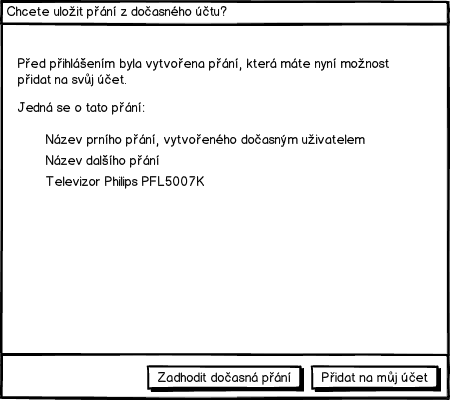
\includegraphics[width=70mm]{./pictures/mock/dialog-pridani-docasnych-prani.png}
\caption{\ref{sc-10}}
\label{fig:dialog-pridani-docasnych-prani}
\end{center}
\end{figure}
% !TEX root = ../DP_Vik_Tomas_2013.tex
\chapter{Dotazník pro vyhodnocení návrhu uživatelského rozhraní}
Popis jakým způsobem se dospělo k navržení následujícího dotazníku je popsán v kapitole \ref{sec:metodika-dotaznik}. Následuje přesné znění dotazníku tak, jak ho obdrželi respondenti. Dotazník byl vytvořen a vyplňován elektronicky pomocí aplikace Google Drive.

\section{Vyhodnocení aplikace WishList}
Ahoj, díky za Tvůj čas, půjde přibližně o 15 min. Teď mi pomůžeš s vyhodnocením návrhu uživatelského rozhraní mojí diplomové práce, tedy jak náročné je ovládat aplikaci WishList. 

NEŽ BUDEŠ POKRAČOVAT V ČTENÍ DOTAZNÍKU, JDI PROSÍM NA STRÁNKU http://tomasvik.cz A 5-10 MINUT NA NÍ PRACUJ. POKUD UŽ TAM NEBUDEŠ MÍT CO DĚLAT, TAK MŮŽEŠ S PRACÍ NA STRÁNCE SKONČIT DŘÍVE. PAK SE VRAŤ K DOTAZNÍKU A VYPLŇ HO.

Ještě jednou díky za Tvůj čas! pánbůh ti to oplatí na dětech

\subsection{Základní dotazník}
Odpověz jak moc se ztotožňuješ s následujícími prohlášeními

\begin{enumerate}
\item \textbf{Myslím že bych rád používal systém častěji} \newline
		Vůbec nesouhlasím |1-2-3-4-5|\footnote{V elektronické verzi je možné zvolit čílo pomocí RadioButton.} Plně souhlasím
\item \textbf{Aplikace mi přišla zbytečně složitá} \newline
		Vůbec nesouhlasím |1-2-3-4-5| Plně souhlasím
\item \textbf{Aplikace se mi snadno používala} \newline
		Vůbec nesouhlasím |1-2-3-4-5| Plně souhlasím
\item \textbf{Myslím že k používání tohoto systému bych potřeboval technicky vzdělaného člověka.} \newline
		Vůbec nesouhlasím |1-2-3-4-5| Plně souhlasím
\item \textbf{Několik funkcí systému mi v aplikaci přišlo dobře umístěno} \newline
		Vůbec nesouhlasím |1-2-3-4-5| Plně souhlasím
\item \textbf{Myslím že v systému bylo příliš nesrovnalostí} \newline
		Vůbec nesouhlasím |1-2-3-4-5| Plně souhlasím
\item \textbf{Dokážu si představit že většina lidí by se naučila používat tuto aplikaci rychle} \newline
		Vůbec nesouhlasím |1-2-3-4-5| Plně souhlasím
\item \textbf{Přišel jsem na to že systém je příliš složitý na používání} \newline
		Vůbec nesouhlasím |1-2-3-4-5| Plně souhlasím
\item \textbf{Cítil jsem se že mi jde ovládání aplikace dobře} \newline
		Vůbec nesouhlasím |1-2-3-4-5| Plně souhlasím
\item \textbf{Potřeboval bych se naučit ještě hodně věcí, než bych mohl používat systém} \newline
		Vůbec nesouhlasím |1-2-3-4-5| Plně souhlasím
\end{enumerate}

\subsection{Pokročilý dotazník}
Jestli už sem tě zdržel moc, nemusíš tyto otázky vyplňovat :)

\begin{enumerate}
\item \textbf{Pochopil/a jsi na co aplikace slouží?} To znamená byl ti jasný účel aplikace? \newline
		vůbec nebo s velkými problémy |1-2-3-4-5| okamžitě bez problému
\item \textbf{Bylo náročné vyhledat předmět přání?} \newline
		nepřišel jsem na to jak |1-2-3-4-5| byla to hračka
\item \textbf{Přihlásil/a, nebo zaregistroval/a jsi se do aplikace?}
		\begin{itemize}
		\item ano
		\item Ne, ale věděl/a jsem že to je možné
		\item ne, nevěděl/a jsem že jde
		\end{itemize}
\item \textbf{Přidal/a jsi přání do svého seznamu?}
		\begin{itemize}
		\item ano, jedno
		\item ano, více
		\item ne
		\end{itemize}
\end{enumerate}

\subsection{Práce s přáními}
\begin{enumerate}
\item \textbf{Zkusil jsi přemístit svá přání v seznamu?} To znamená přesunout jedno nad druhé a tím mu změnit prioritu?
		\begin{itemize}
		\item ano
		\item ne
		\end{itemize}
\item \textbf{Všiml/a jsi si panelu se štítky?} V levé části stránky byl seznam štítků, všiml/a jsi si ho?
		\begin{itemize}
		\item ano
		\item ne
		\end{itemize}
\item \textbf{Použil/a jsi seznam štítků k filtrování tvých přání?} Klikl/a jsi na nějaký štítek a tím si zobrazil/a pouze přání označená tímto štítkem?
		\begin{itemize}
		\item ano
		\item ne
		\end{itemize}
\end{enumerate}

\subsection{Práce s přáními}
\begin{enumerate}
\item \textbf{Vybral/a jsi si vlastní obrázek k přání při jeho přidávání?}
		\begin{itemize}
		\item Ano
		\item Ne, ale věděl/a jsem že to je možné
		\item Ne, nevěděl/a jsem že to jde
		\end{itemize}
\item \textbf{Vybral/a jsis vlastní obrázek k přání při jeho přidávání?}
		\begin{itemize}
		\item Ano
		\item Ne, ale věděl/a jsem že to je možné
		\item Ne, nevěděl/a jsem že to jde
		\end{itemize}
\item \textbf{Smazal/a jsi nějaké přání ze svého seznamu?}
		\begin{itemize}
		\item Ano
		\item Ne, ale věděl/a jsem že to je možné
		\item Ne, nevěděl/a jsem že to jde
		\end{itemize}
\item \textbf{Zobrazil/a jsi detail nebo upravil/a jsi nějaké prání?} To znamená kliknout na přání v seznamu přání a zobrazit si tím obrazovku detil přání, která vypadá podobně jako při přidávání přání.
		\begin{itemize}
		\item Ano
		\item Ne, ale věděl/a jsem že to je možné
		\item Ne, nevěděl/a jsem že to jde
		\end{itemize}
\item \textbf{Označil/a jsi nějaké své přání jako splněné?}
		\begin{itemize}
		\item Ano
		\item Ne, ale věděl/a jsem že to je možné
		\item Ne, nevěděl/a jsem že to jde
		\end{itemize}
\item \textbf{Přidal/a jsi k nějakému přání při vytváření štítek?} To znamená vložit při vytváření přání do seznamu štítků nějaké hodnoty, čímž ho vlastně zařadit do kategorie se stejným názvem jako má štítek.
		\begin{itemize}
		\item Ano
		\item Ne, ale věděl/a jsem že to je možné
		\item Ne, nevěděl/a jsem že to jde
		\end{itemize}
\end{enumerate}

\subsection{Toto je poslední stránka dotazníku}
\textbf{Napadlo, překvapilo, naštvalo, nebo potěšilo tě něco při práci s aplikací?} Prosím napiš mi to sem.
\newline
\newline
\newline
\newline

\subsection{Stránka s potvrzením odeslání dotazníku}
Toto se zobrazilo uživateli, který odeslal dotazník:

Tvoje odpovědi byly zaznamenány a já je zapracuji do výsledků své práce. Ještě poslední díky za Tvůj čas. Pokud by tě náhodou zajímaly výsledky, ozvi se na vicek22@gmail.com.
% !TEX root = ../DP_Vik_Tomas_2013.tex
\chapter{Výsledky dotazníku pro vyhodnocení UI}
\label{chp:vysledky}
V této příloze jsou pouze čistě výsledky dotazníku, jejich vyhodnocení se nachází v kapitole \ref{sec:vyhodnoceni-dotazniku}. Ve schématech znamenají tučná čísla počet respondentů. Celkem jich bylo \textbf{22}.

\section{Základní dotazník}
Výsledky odpovědí na základní SUS dotazník.
Všechny odpovědi jsou hodnocené na stupnici 1-Vůbec nesouhlasím až 5-Plně souhlasím.

\begin{figure}[H]
\begin{center}
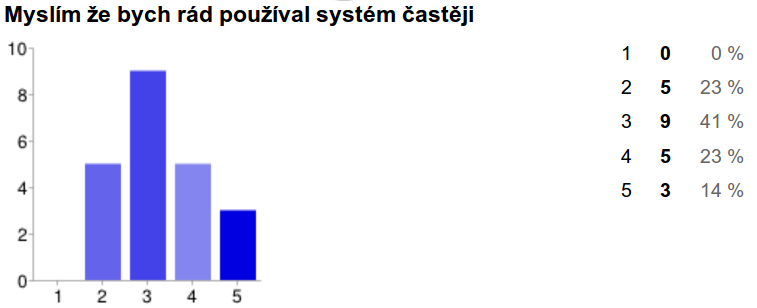
\includegraphics[width=80mm]{./pictures/dotaznik/sus-01.png}
%\caption{Graf s výsledky první otázky}
\label{fig:dot:sus-01}
\end{center}
\end{figure}

\begin{figure}[H]
\begin{center}
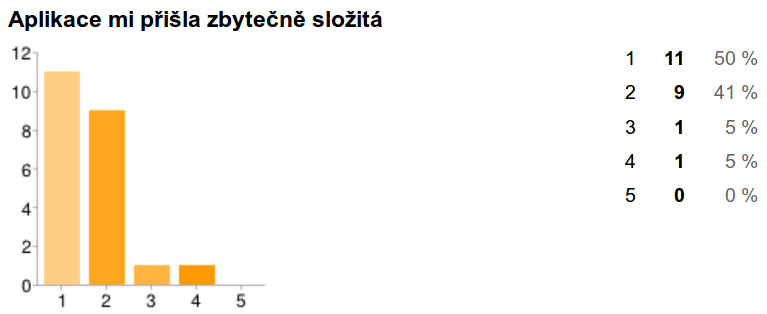
\includegraphics[width=80mm]{./pictures/dotaznik/sus-02.png}
%\caption{Graf s výsledky druhé otázky}
\label{fig:dot:sus-02}
\end{center}
\end{figure}

\begin{figure}[H]
\begin{center}
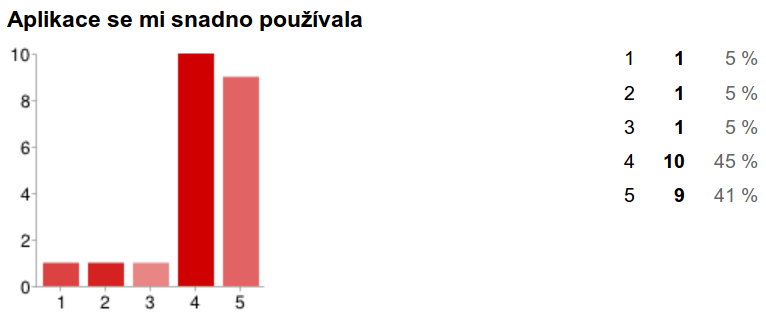
\includegraphics[width=80mm]{./pictures/dotaznik/sus-03.png}
%\caption{Graf s výsledky třetí otázky}
\label{fig:dot:sus-03}
\end{center}
\end{figure}

\begin{figure}[H]
\begin{center}
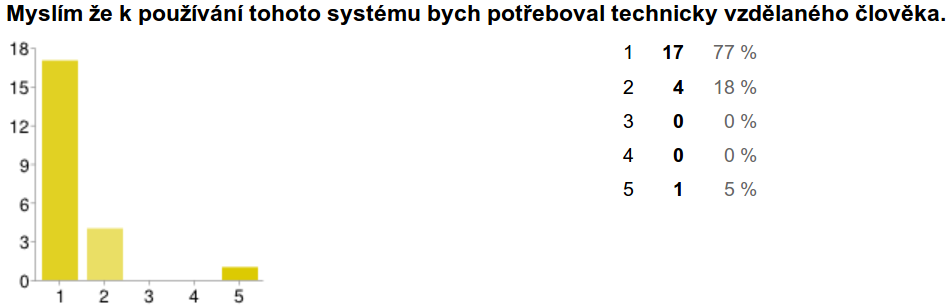
\includegraphics[width=80mm]{./pictures/dotaznik/sus-04.png}
%\caption{Graf s výsledky čtvrté otázky}
\label{fig:dot:sus-04}
\end{center}
\end{figure}

\begin{figure}[H]
\begin{center}
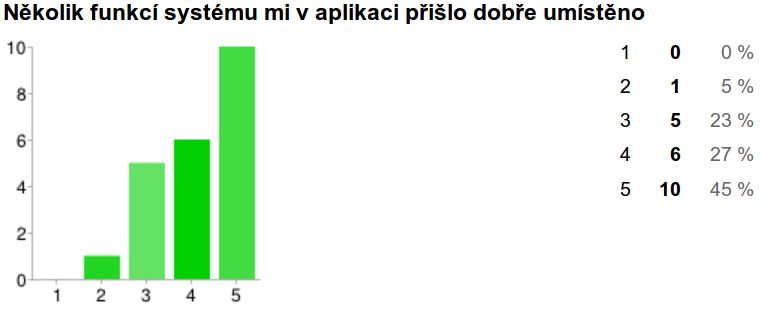
\includegraphics[width=80mm]{./pictures/dotaznik/sus-05.png}
%\caption{Graf s výsledky páté otázky}
\label{fig:dot:sus-05}
\end{center}
\end{figure}

\begin{figure}[H]
\begin{center}
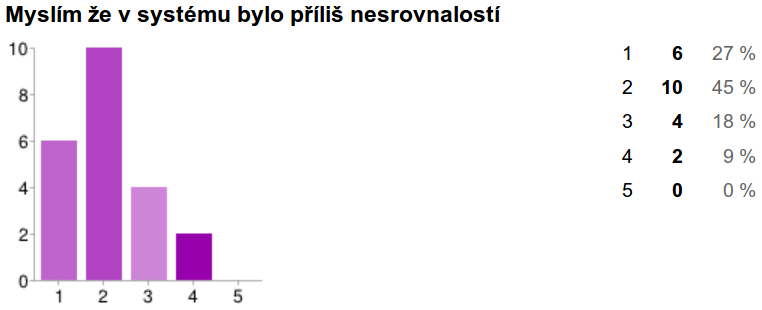
\includegraphics[width=80mm]{./pictures/dotaznik/sus-06.png}
%\caption{Graf s výsledky šesté otázky}
\label{fig:dot:sus-06}
\end{center}
\end{figure}

\begin{figure}[H]
\begin{center}
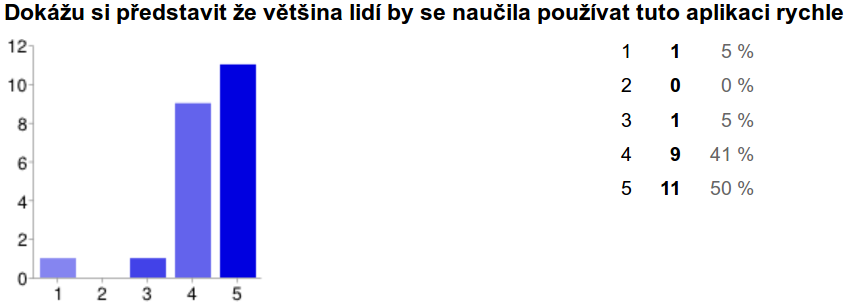
\includegraphics[width=80mm]{./pictures/dotaznik/sus-07.png}
%\caption{Graf s výsledky sedmé otázky}
\label{fig:dot:sus-07}
\end{center}
\end{figure}

\begin{figure}[H]
\begin{center}
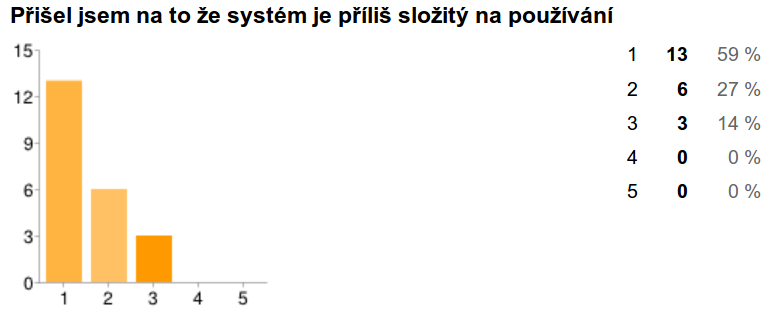
\includegraphics[width=80mm]{./pictures/dotaznik/sus-08.png}
%\caption{Graf s výsledky osmé otázky}
\label{fig:dot:sus-08}
\end{center}
\end{figure}

\begin{figure}[H]
\begin{center}
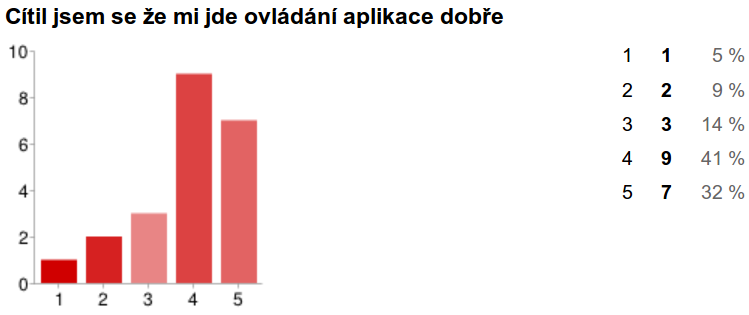
\includegraphics[width=80mm]{./pictures/dotaznik/sus-09.png}
%\caption{Graf s výsledky deváté otázky}
\label{fig:dot:sus-09}
\end{center}
\end{figure}

\begin{figure}[H]
\begin{center}
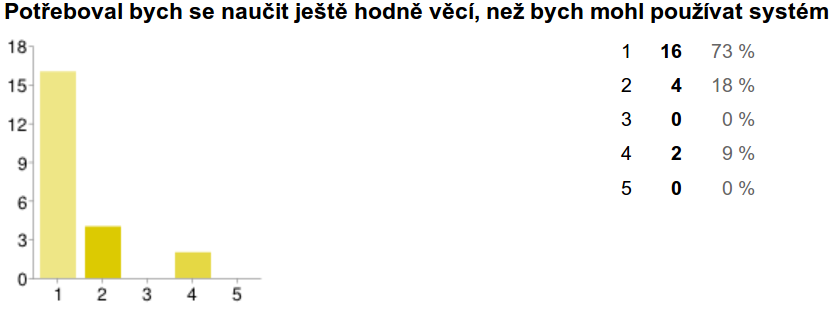
\includegraphics[width=80mm]{./pictures/dotaznik/sus-10.png}
%\caption{Graf s výsledky desáté otázky}
\label{fig:dot:sus-10}
\end{center}
\end{figure}

\section{Pokročilý dotazník}
U otázky \emph{Pochopil jsi na co aplikace slouží?} znamenají odpovědi 1=vůbec nebo s velkými problémy až 5=okamžitě bez problému. U otázky \emph{Bylo náročné přidat předmět přání?} znamenají odpověďi 1=nepřišel jsem na to jak až 5=byla to hračka.
Od výsledků poslední otázky se odvíjelo, na jaké další otázky bude uživatel odpovídat (např. pokud uživatel nepřidal ani jedno přání, nemá smysl se ho ptát na to zdali přesouval přání ve svém seznamu). Proto je tato část poslední, kde odpovídalo všech 22 respondentů.

\begin{figure}[H]
\begin{center}
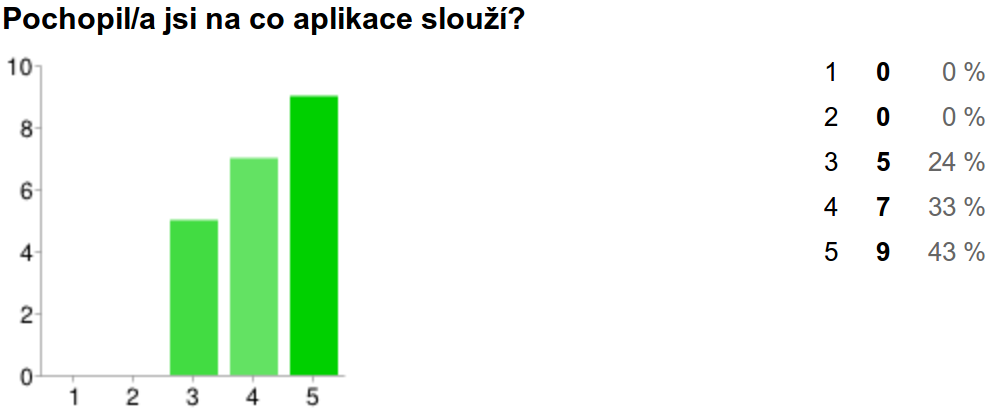
\includegraphics[width=80mm]{./pictures/dotaznik/pokrocily-01.png}
\label{fig:dot:pokrocily-01}
\end{center}
\end{figure}

\begin{figure}[H]
\begin{center}
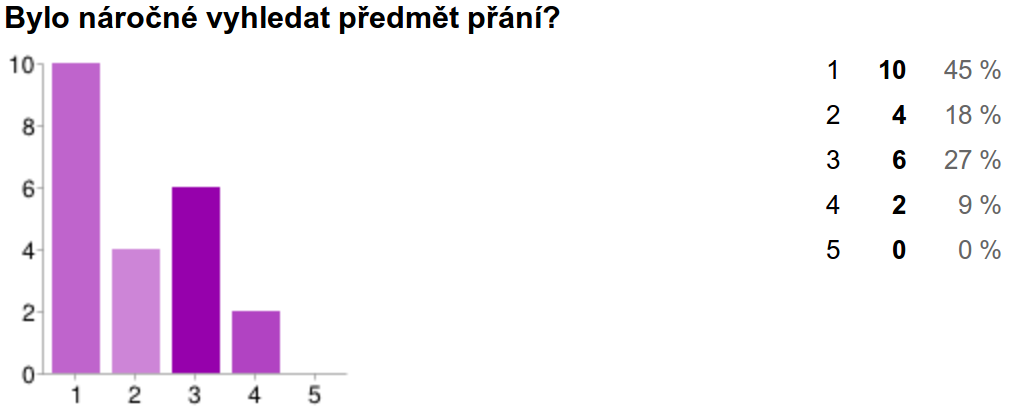
\includegraphics[width=80mm]{./pictures/dotaznik/pokrocily-02.png}
\label{fig:dot:pokrocily-02}
\end{center}
\end{figure}

\begin{figure}[H]
\begin{center}
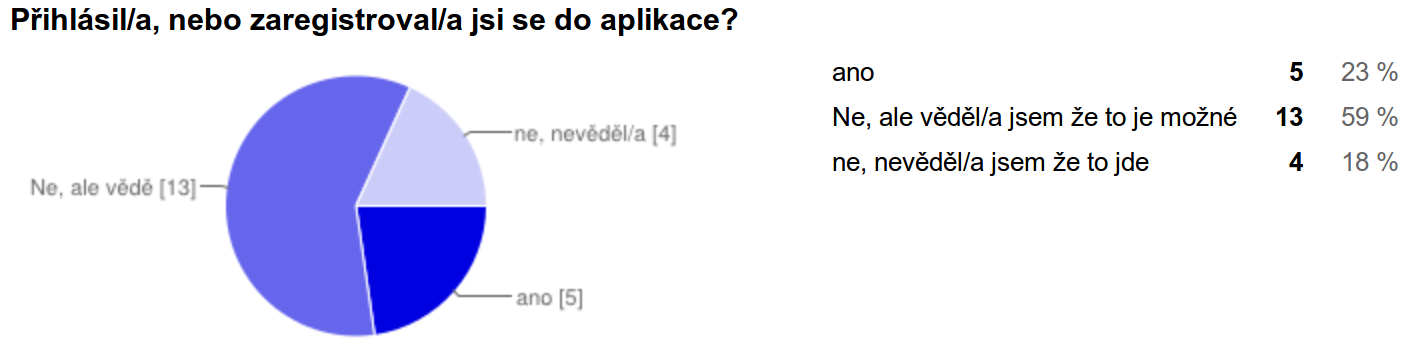
\includegraphics[width=120mm]{./pictures/dotaznik/pokrocily-03.png}
\label{fig:dot:pokrocily-03}
\end{center}
\end{figure}

\begin{figure}[H]
\begin{center}
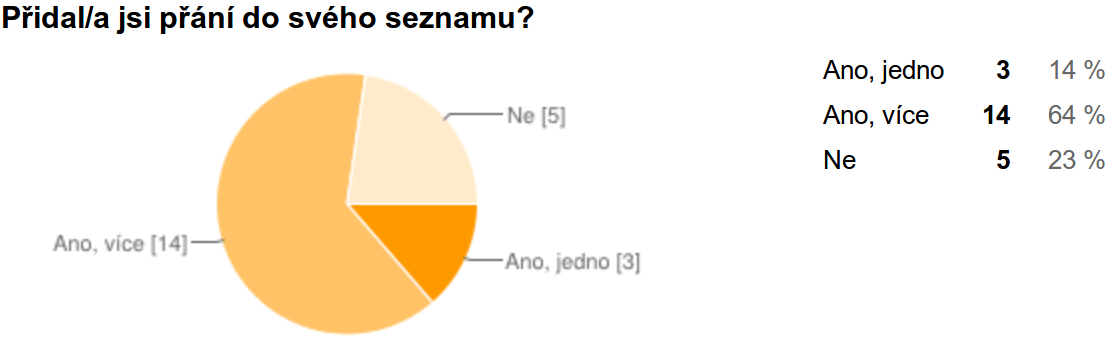
\includegraphics[width=100mm]{./pictures/dotaznik/pokrocily-04.png}
\label{fig:dot:pokrocily-04}
\end{center}
\end{figure}


\section{Práce s přáními}
Do této kategorie přispívali pouze respondenti, kteří v předchozí části dotazníku odpověděli, že do svého seznamu přidali více než jedno přání.
\begin{figure}[H]
\begin{center}
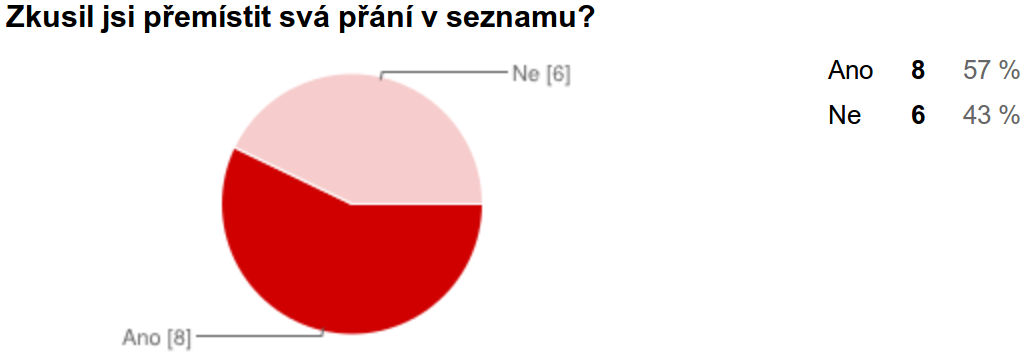
\includegraphics[width=110mm]{./pictures/dotaznik/vice-prani-01.png}
\label{fig:dot:vice-prani-01}
\end{center}
\end{figure}

\begin{figure}[H]
\begin{center}
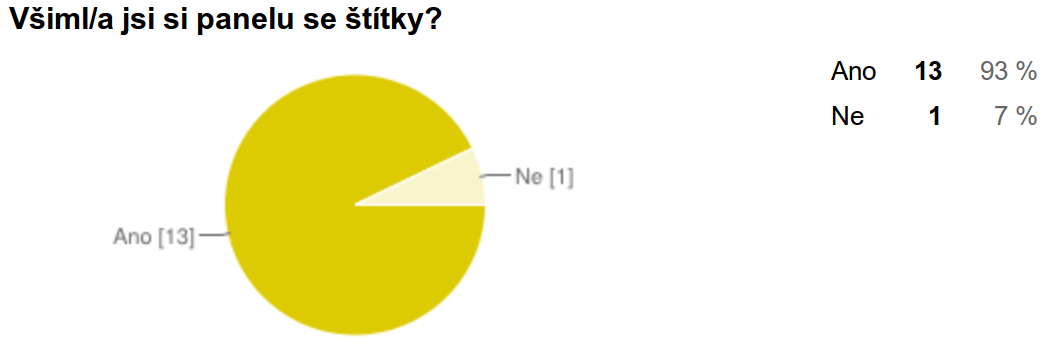
\includegraphics[width=110mm]{./pictures/dotaznik/vice-prani-02.png}
\label{fig:dot:vice-prani-02}
\end{center}
\end{figure}

\begin{figure}[H]
\begin{center}
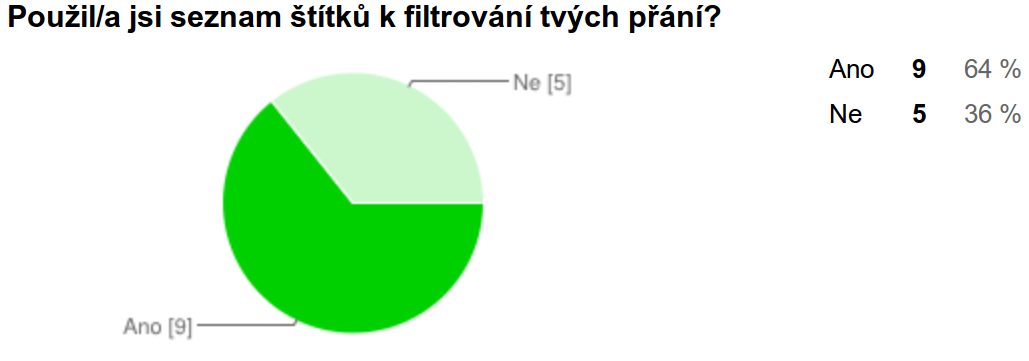
\includegraphics[width=110mm]{./pictures/dotaznik/vice-prani-03.png}
\label{fig:dot:vice-prani-03}
\end{center}
\end{figure}

\section{Práce s přáním}
\begin{figure}[H]
\begin{center}
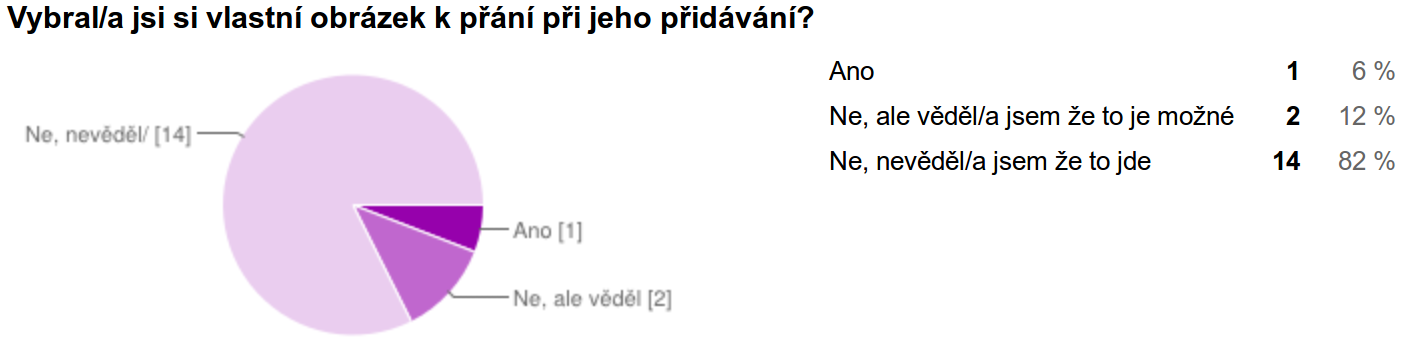
\includegraphics[width=110mm]{./pictures/dotaznik/jedno-prani-01.png}
\label{fig:dot:jedno-prani-01}
\end{center}
\end{figure}

\begin{figure}[H]
\begin{center}
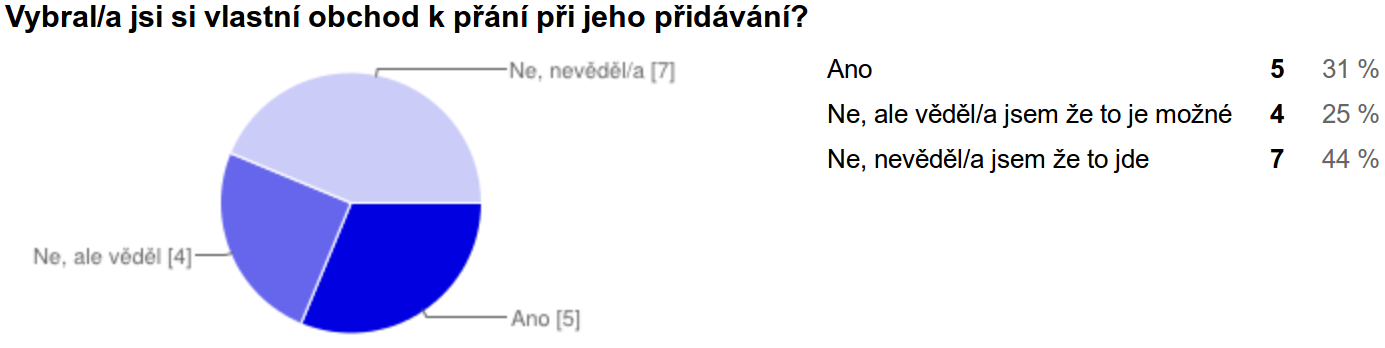
\includegraphics[width=110mm]{./pictures/dotaznik/jedno-prani-02.png}
\label{fig:dot:jedno-prani-02}
\end{center}
\end{figure}

\begin{figure}[H]
\begin{center}
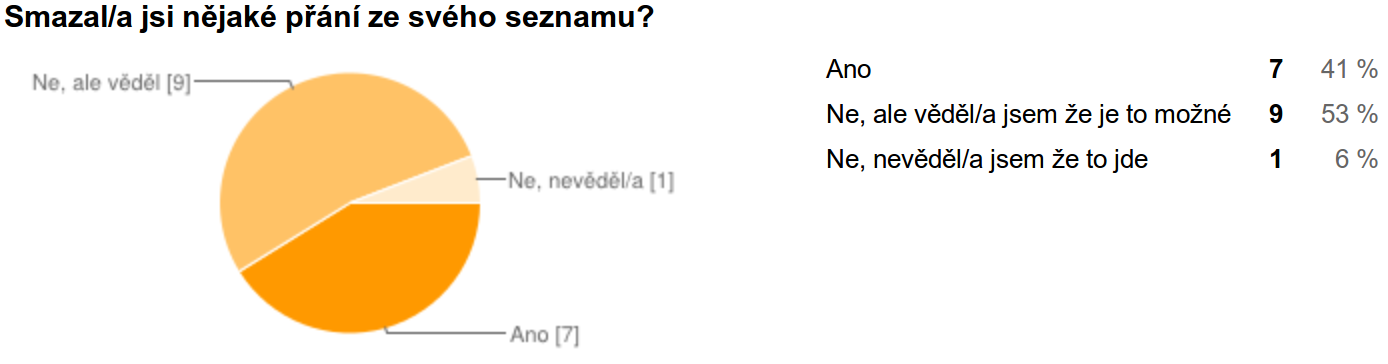
\includegraphics[width=110mm]{./pictures/dotaznik/jedno-prani-03.png}
\label{fig:dot:jedno-prani-03}
\end{center}
\end{figure}

\begin{figure}[H]
\begin{center}
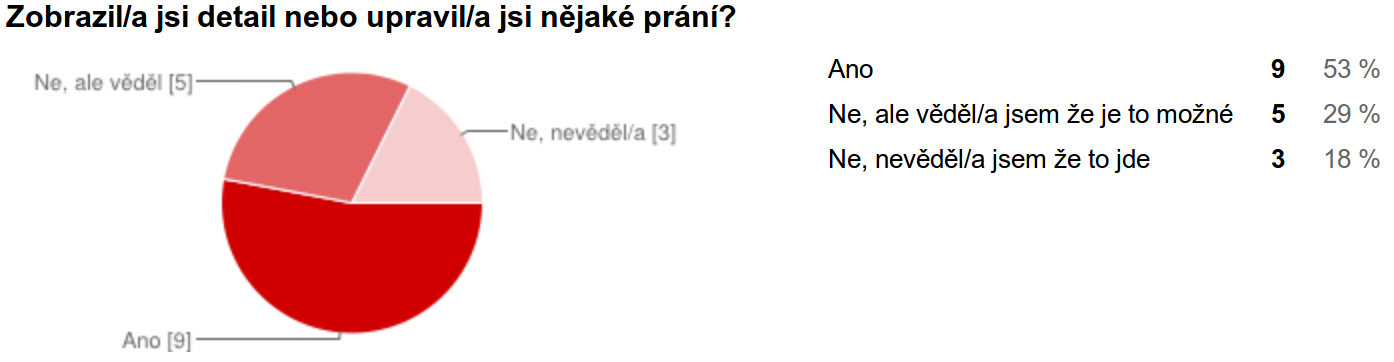
\includegraphics[width=110mm]{./pictures/dotaznik/jedno-prani-04.png}
\label{fig:dot:jedno-prani-04}
\end{center}
\end{figure}

\begin{figure}[H]
\begin{center}
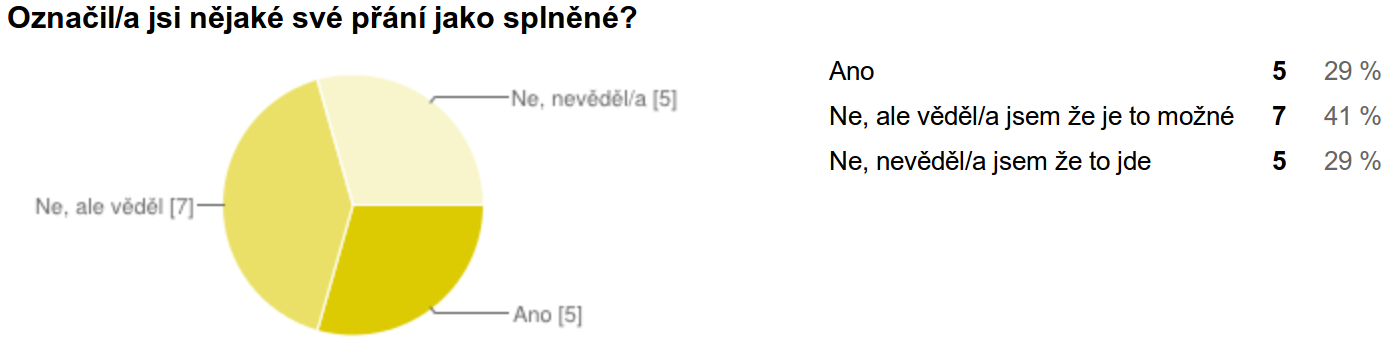
\includegraphics[width=110mm]{./pictures/dotaznik/jedno-prani-05.png}
\label{fig:dot:jedno-prani-05}
\end{center}
\end{figure}

\begin{figure}[H]
\begin{center}
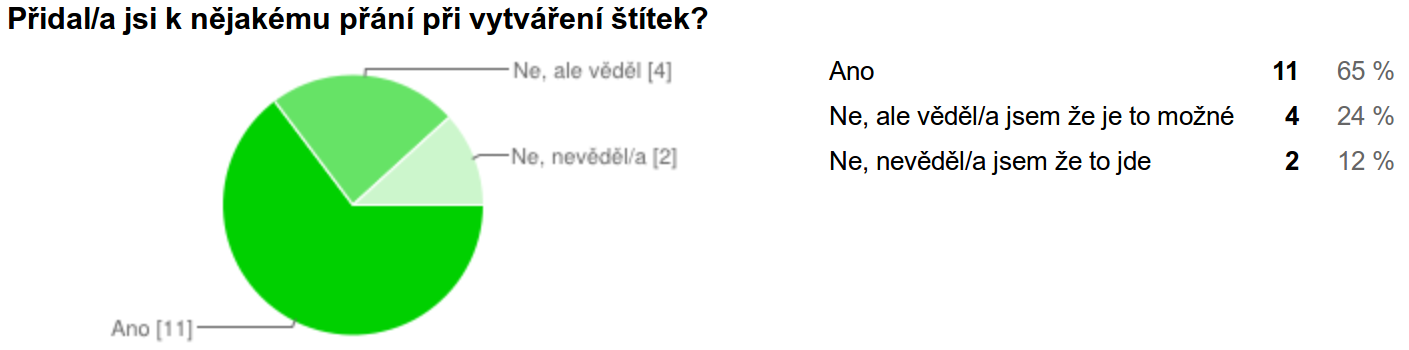
\includegraphics[width=110mm]{./pictures/dotaznik/jedno-prani-06.png}
\label{fig:dot:jedno-prani-06}
\end{center}
\end{figure}
% !TEX root = ../DP_Vik_Tomas_2013.tex
\chapter{Jednoduchý překlad Nielsenovy heuristiky}
V této příloze je přeložen význam deseti klíčových bodů Nielsenovy heuristiky.
\begin{enumerate}
\item \textbf{viditelnost stavu systému} – systém by měl být schopen uživateli vždy poskytnout v dostatečně krátkém časovém horizontu srozumitelnou zpětnou vazbu o svém stavu, aby hodnotitel věděl, co se systémem právě provádí\cite{thesis:flamik} 

\item \textbf{shoda systému a reálného světa} – systém by měl hovořit uživatelským jazykem. Měl by používat slova a fráze uživatelsky známé a neměl by naopak využívat obraty a slova, která mají srozumitelný význam jen pro návrháře a jeho autory. Dále by měl využívat zvyklosti reálného světa a informace zobrazovat v logickém pořadí\cite{thesis:flamik} 

\item \textbf{svobodné akce uživatele} – uživatel je schopen omylem si zvolit funkci systému, kterou nepotřebuje. Proto je nutné jasně naznačit „únikové místo“ pro rychlé opuštění z nechtěného stavu a to bez nutnosti komplikovaného dialogu se systémem. Z tohoto důvodu by měl systém poskytovat funkce typu „Zpět“ a „Znovu“\cite{thesis:flamik} 

\item \textbf{konzistence a standardy} – uživatel by neměl být nucen přemýšlet, zda různé situace, akce nebo slova znamenají totéž. Systém byse měl řídit konvencemi dané platformy\cite{thesis:flamik} 

\item \textbf{prevence chyb} - je lepší mít systém, který předchází chybám, než systém, který chyby pouze ohlašuje chybovými zprávami\cite{thesis:flamik} 

\item \textbf{preference rozpoznání před vzpomínáním} – veškeré objekty a volby akcí systému musí být viditelné a srozumitelné. Uživatel by neměl být nucen pamatovat si informace z jedné části dialogu se systémem pro práci s další částí systému. Návod k používání systému by měl být v případě potřeby snadno dostupný\cite{thesis:flamik} 

\item \textbf{flexibilita a efektivnost použití} – nástroje k urychlení práce se systémem by měly být k dispozici pro zkušené uživatele. Pro nováčky by však měly být skryté. Systém by měl být přizpůsobivý z hlediska rychlosti a snadnosti ovládání jak pro začátečníky, tak pro časté a zkušené uživatele. Uživatel by měl mít tedy rychlý přístup k těm funkcím systému, které často využívá, proto by se měla rozlišovat podpora pro různé uživatele\cite{thesis:flamik} 

\item \textbf{efektivní informační design} – dialog by neměl obsahovat informace, které nejsou podstatné pro funkci systému nebo jsou potřeba jen zřídka. Každá nadbytečná informace soupeří o pozornost uživatele s informacemi podstatnými a snižuje jejich relativní viditelnost. Krátké řádky a odstavce jsou čitelnější. Grafy, tabulky,seznamy jsou reprezentativnější než rozsáhlý popis v uceleném textu\cite{thesis:flamik} 

\item \textbf{pomoc při rozpoznávání, stanovení chyb a následné zotavení} – zpráva o chybě systému by neměla být vyjádřena v heslech či kódech, ale v přirozeném jazyce vystihující daný problém a s konstruktivní nabídkou k řešení problému\cite{thesis:flamik} 

\item \textbf{nápověda a dokumentace orientovaná na úkoly} – ideálním systémem je takový systém, který ke svému používání nepotřebuje žádnou nápovědu ani dokumentaci, ale měl by ho však vždy obsahovat. Každá informace v tomto dokumentu by měla být snadno dohledatelná. Měl by se zaměřovat na pomoc při řešení úkolů, které uživatel provádí nebo chce provést a měl by také obsahovat konkrétní kroky k jejich provedení. Neměl by být však příliš obsáhlý.\cite{thesis:flamik}

\end{enumerate}
% !TEX root = ../DP_Vik_Tomas_2013.tex
\chapter{Instalační příručka}
Aplikace je dostupná online na adrese \url{http://tomasvik.cz} a zároveň jsou její zdrojové kódy přiloženy na CD dodávaném k této práci. Následuje postup, jak nainstalovat aplikaci na lokálním přostředí.

\section{Instalace aplikace na lokálním prostředí}
Tento postup je určený pro linuxové systémy, konkrétně systémy odvozené z distribuce Debian. Zprovoznění aplikace na jiném linuxovém systému by neměl být žádný problém. Pro zprovoznění na windows doporučuji \url{http://railsinstaller.org/} na který jsou nejlepší odezvy co se týče instalace rails.

Přestože nejsou známy problémy, které by mohly nastat při instalaci na Windows, platí následující:

\textbf{Jediným zaručeně podporovaným operačním systémem je linux s APT balíčkovacím systémem.} Aplikace byla testována a vývíjena na systému Ubuntu 12.04 LTS.

Nejdříve je důležité mít nainstalovaný balík ruby ve verzi 1.9.2 a vyšší

\lstset{language = bash, style=custom}
\begin{lstlisting}
sudo apt-get install ruby1.9.3
\end{lstlisting}

pokud příkaz

\begin{lstlisting}
ruby --version
\end{lstlisting}

nevrátí správnou verzi, je potřeba tuto verzi nastavit příkazem

\begin{lstlisting}
sudo update-alternatives --config ruby
\end{lstlisting}

poté stačí nainstalovat bundler, pokud ještě není nainstalovaný

\begin{lstlisting}
sudo gem install bundler
\end{lstlisting}

přepnout se do adrésáře zdrojových kódů diplomové práce

\begin{lstlisting}
cd ~/wishlist
\end{lstlisting}

a nainstalovat vše potřebné příkazem

\begin{lstlisting}
sudo bundle install
\end{lstlisting}

nyní stačí inicializovat databázi práce

\begin{lstlisting}
rake db:setup
\end{lstlisting}

a spusti aplikaci pomocí příkazu 

\begin{lstlisting}
rails s
\end{lstlisting}

Nyní je možné aplikaci nalézt na adrese \url{http://localhost:3000}




\chapter{Obsah přiloženého CD}

%upravte podle skutecnosti

\begin{figure}
	\dirtree{%
		.1 readme.txt\DTcomment{stručný popis obsahu CD}.
    .1 src\DTcomment{adresář se zdrojovými kódy práce}.
    .2 wishlist\DTcomment{adresář se zdrojovými kódy implementace}.
		.2 lib\DTcomment{adresář s Java Script knihovnami použitými při implementaci}.
		.2 thesis\DTcomment{zdrojová forma práce ve formátu \LaTeX{}}.
		.1 text\DTcomment{text práce}.
    .2 DP\_Vik\_Tomas\_2013.pdf\DTcomment{text práce ve formátu PDF}.
    .2 DP\_Vik\_Tomas\_2013.ps\DTcomment{text práce ve formátu PS}.
	}
\end{figure}

\end{document}
